\documentclass[1p]{elsarticle_modified}
%\bibliographystyle{elsarticle-num}

%\usepackage[colorlinks]{hyperref}
%\usepackage{abbrmath_seonhwa} %\Abb, \Ascr, \Acal ,\Abf, \Afrak
\usepackage{amsfonts}
\usepackage{amssymb}
\usepackage{amsmath}
\usepackage{amsthm}
\usepackage{scalefnt}
\usepackage{amsbsy}
\usepackage{kotex}
\usepackage{caption}
\usepackage{subfig}
\usepackage{color}
\usepackage{graphicx}
\usepackage{xcolor} %% white, black, red, green, blue, cyan, magenta, yellow
\usepackage{float}
\usepackage{setspace}
\usepackage{hyperref}

\usepackage{tikz}
\usetikzlibrary{arrows}

\usepackage{multirow}
\usepackage{array} % fixed length table
\usepackage{hhline}

%%%%%%%%%%%%%%%%%%%%%
\makeatletter
\renewcommand*\env@matrix[1][\arraystretch]{%
	\edef\arraystretch{#1}%
	\hskip -\arraycolsep
	\let\@ifnextchar\new@ifnextchar
	\array{*\c@MaxMatrixCols c}}
\makeatother %https://tex.stackexchange.com/questions/14071/how-can-i-increase-the-line-spacing-in-a-matrix
%%%%%%%%%%%%%%%

\usepackage[normalem]{ulem}

\newcommand{\msout}[1]{\ifmmode\text{\sout{\ensuremath{#1}}}\else\sout{#1}\fi}
%SOURCE: \msout is \stkout macro in https://tex.stackexchange.com/questions/20609/strikeout-in-math-mode

\newcommand{\cancel}[1]{
	\ifmmode
	{\color{red}\msout{#1}}
	\else
	{\color{red}\sout{#1}}
	\fi
}

\newcommand{\add}[1]{
	{\color{blue}\uwave{#1}}
}

\newcommand{\replace}[2]{
	\ifmmode
	{\color{red}\msout{#1}}{\color{blue}\uwave{#2}}
	\else
	{\color{red}\sout{#1}}{\color{blue}\uwave{#2}}
	\fi
}

\newcommand{\Sol}{\mathcal{S}} %segment
\newcommand{\D}{D} %diagram
\newcommand{\A}{\mathcal{A}} %arc


%%%%%%%%%%%%%%%%%%%%%%%%%%%%%5 test

\def\sl{\operatorname{\textup{SL}}(2,\Cbb)}
\def\psl{\operatorname{\textup{PSL}}(2,\Cbb)}
\def\quan{\mkern 1mu \triangleright \mkern 1mu}

\theoremstyle{definition}
\newtheorem{thm}{Theorem}[section]
\newtheorem{prop}[thm]{Proposition}
\newtheorem{lem}[thm]{Lemma}
\newtheorem{ques}[thm]{Question}
\newtheorem{cor}[thm]{Corollary}
\newtheorem{defn}[thm]{Definition}
\newtheorem{exam}[thm]{Example}
\newtheorem{rmk}[thm]{Remark}
\newtheorem{alg}[thm]{Algorithm}

\newcommand{\I}{\sqrt{-1}}
\begin{document}

%\begin{frontmatter}
%
%\title{Boundary parabolic representations of knots up to 8 crossings}
%
%%% Group authors per affiliation:
%\author{Yunhi Cho} 
%\address{Department of Mathematics, University of Seoul, Seoul, Korea}
%\ead{yhcho@uos.ac.kr}
%
%
%\author{Seonhwa Kim} %\fnref{s_kim}}
%\address{Center for Geometry and Physics, Institute for Basic Science, Pohang, 37673, Korea}
%\ead{ryeona17@ibs.re.kr}
%
%\author{Hyuk Kim}
%\address{Department of Mathematical Sciences, Seoul National University, Seoul 08826, Korea}
%\ead{hyukkim@snu.ac.kr}
%
%\author{Seokbeom Yoon}
%\address{Department of Mathematical Sciences, Seoul National University, Seoul, 08826,  Korea}
%\ead{sbyoon15@snu.ac.kr}
%
%\begin{abstract}
%We find all boundary parabolic representation of knots up to 8 crossings.
%
%\end{abstract}
%\begin{keyword}
%    \MSC[2010] 57M25 
%\end{keyword}
%
%\end{frontmatter}

%\linenumbers
%\tableofcontents
%
\newcommand\colored[1]{\textcolor{white}{\rule[-0.35ex]{0.8em}{1.4ex}}\kern-0.8em\color{red} #1}%
%\newcommand\colored[1]{\textcolor{white}{ #1}\kern-2.17ex	\textcolor{white}{ #1}\kern-1.81ex	\textcolor{white}{ #1}\kern-2.15ex\color{red}#1	}

{\Large $\underline{12a_{0711}~(K12a_{0711})}$}

\setlength{\tabcolsep}{10pt}
\renewcommand{\arraystretch}{1.6}
\vspace{1cm}\begin{tabular}{m{100pt}>{\centering\arraybackslash}m{274pt}}
\multirow{5}{120pt}{
	\centering
	\includegraphics[width=112pt]{../../../GIT/diagram.site/Diagrams/png/1512_12a_0711.png}\\
\ \ \ A knot diagram\footnotemark}&
\allowdisplaybreaks
\textbf{Linearized knot diagam} \\
\cline{2-2}
 &
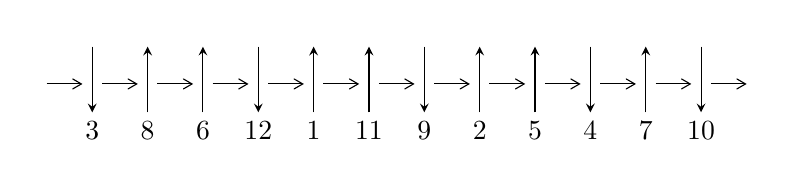
\begin{tikzpicture}[x=20pt, y=17pt]
	% nodes
	\node (C0) at (0, 0) {};
	\node (C1) at (1, 0) {};
	\node (C1U) at (1, +1) {};
	\node (C1D) at (1, -1) {3};

	\node (C2) at (2, 0) {};
	\node (C2U) at (2, +1) {};
	\node (C2D) at (2, -1) {8};

	\node (C3) at (3, 0) {};
	\node (C3U) at (3, +1) {};
	\node (C3D) at (3, -1) {6};

	\node (C4) at (4, 0) {};
	\node (C4U) at (4, +1) {};
	\node (C4D) at (4, -1) {12};

	\node (C5) at (5, 0) {};
	\node (C5U) at (5, +1) {};
	\node (C5D) at (5, -1) {1};

	\node (C6) at (6, 0) {};
	\node (C6U) at (6, +1) {};
	\node (C6D) at (6, -1) {11};

	\node (C7) at (7, 0) {};
	\node (C7U) at (7, +1) {};
	\node (C7D) at (7, -1) {9};

	\node (C8) at (8, 0) {};
	\node (C8U) at (8, +1) {};
	\node (C8D) at (8, -1) {2};

	\node (C9) at (9, 0) {};
	\node (C9U) at (9, +1) {};
	\node (C9D) at (9, -1) {5};

	\node (C10) at (10, 0) {};
	\node (C10U) at (10, +1) {};
	\node (C10D) at (10, -1) {4};

	\node (C11) at (11, 0) {};
	\node (C11U) at (11, +1) {};
	\node (C11D) at (11, -1) {7};

	\node (C12) at (12, 0) {};
	\node (C12U) at (12, +1) {};
	\node (C12D) at (12, -1) {10};
	\node (C13) at (13, 0) {};

	% arrows
	\draw[->,>={angle 60}]
	(C0) edge (C1) (C1) edge (C2) (C2) edge (C3) (C3) edge (C4) (C4) edge (C5) (C5) edge (C6) (C6) edge (C7) (C7) edge (C8) (C8) edge (C9) (C9) edge (C10) (C10) edge (C11) (C11) edge (C12) (C12) edge (C13) ;	\draw[->,>=stealth]
	(C1U) edge (C1D) (C2D) edge (C2U) (C3D) edge (C3U) (C4U) edge (C4D) (C5D) edge (C5U) (C6D) edge (C6U) (C7U) edge (C7D) (C8D) edge (C8U) (C9D) edge (C9U) (C10U) edge (C10D) (C11D) edge (C11U) (C12U) edge (C12D) ;
	\end{tikzpicture} \\
\hhline{~~} \\& 
\textbf{Solving Sequence} \\ \cline{2-2} 
 &
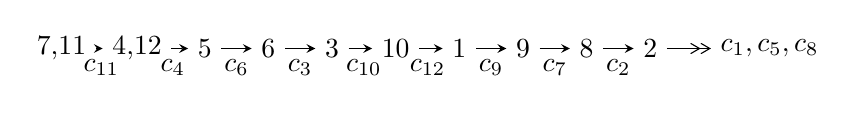
\begin{tikzpicture}[x=23pt, y=7pt]
	% node
	\node (A0) at (-1/8, 0) {7,11};
	\node (A1) at (17/16, 0) {4,12};
	\node (A2) at (17/8, 0) {5};
	\node (A3) at (25/8, 0) {6};
	\node (A4) at (33/8, 0) {3};
	\node (A5) at (41/8, 0) {10};
	\node (A6) at (49/8, 0) {1};
	\node (A7) at (57/8, 0) {9};
	\node (A8) at (65/8, 0) {8};
	\node (A9) at (73/8, 0) {2};
	\node (C1) at (1/2, -1) {$c_{11}$};
	\node (C2) at (13/8, -1) {$c_{4}$};
	\node (C3) at (21/8, -1) {$c_{6}$};
	\node (C4) at (29/8, -1) {$c_{3}$};
	\node (C5) at (37/8, -1) {$c_{10}$};
	\node (C6) at (45/8, -1) {$c_{12}$};
	\node (C7) at (53/8, -1) {$c_{9}$};
	\node (C8) at (61/8, -1) {$c_{7}$};
	\node (C9) at (69/8, -1) {$c_{2}$};
	\node (A10) at (11, 0) {$c_{1},c_{5},c_{8}$};

	% edge
	\draw[->,>=stealth]	
	(A0) edge (A1) (A1) edge (A2) (A2) edge (A3) (A3) edge (A4) (A4) edge (A5) (A5) edge (A6) (A6) edge (A7) (A7) edge (A8) (A8) edge (A9) ;
	\draw[->>,>={angle 60}]	
	(A9) edge (A10);
\end{tikzpicture} \\ 

\end{tabular} \\

\footnotetext{
The image of knot diagram is generated by the software ``\textbf{Draw programme}" developed by Andrew Bartholomew(\url{http://www.layer8.co.uk/maths/draw/index.htm\#Running-draw}), where we modified some parts for our purpose(\url{https://github.com/CATsTAILs/LinksPainter}).
}\phantom \\ \newline 
\centering \textbf{Ideals for irreducible components\footnotemark of $X_{\text{par}}$} 
 
\begin{align*}
I^u_{1}&=\langle 
8.24922\times10^{742} u^{150}-6.55529\times10^{743} u^{149}+\cdots+3.04139\times10^{743} b-5.19965\times10^{746},\\
\phantom{I^u_{1}}&\phantom{= \langle  }-1.91365\times10^{744} u^{150}+1.50999\times10^{745} u^{149}+\cdots+2.56085\times10^{745} a+1.17408\times10^{748},\\
\phantom{I^u_{1}}&\phantom{= \langle  }u^{151}-9 u^{150}+\cdots-77784 u+6736\rangle \\
I^u_{2}&=\langle 
- u^{37}- u^{36}+\cdots+b-1,\;6999926753 u^{38}+2532872060 u^{37}+\cdots+288793 a-11032994937,\\
\phantom{I^u_{2}}&\phantom{= \langle  }u^{39}+u^{38}+\cdots- u-1\rangle \\
I^u_{3}&=\langle 
-85 a^8-32 a^7-448 a^6-448 a^5-2000 a^4+136 a^3-192 a^2+6925 b-2531 a+6968,\\
\phantom{I^u_{3}}&\phantom{= \langle  }a^9+2 a^8+5 a^7+8 a^6+23 a^5+32 a^4+14 a^3+64 a^2+45 a+19,\;u+1\rangle \\
\\
\end{align*}
\raggedright * 3 irreducible components of $\dim_{\mathbb{C}}=0$, with total 199 representations.\\
\footnotetext{All coefficients of polynomials are rational numbers. But the coefficients are sometimes approximated in decimal forms when there is not enough margin.}
\newpage
\renewcommand{\arraystretch}{1}
\centering \section*{I. $I^u_{1}= \langle 8.25\times10^{742} u^{150}-6.56\times10^{743} u^{149}+\cdots+3.04\times10^{743} b-5.20\times10^{746},\;-1.91\times10^{744} u^{150}+1.51\times10^{745} u^{149}+\cdots+2.56\times10^{745} a+1.17\times10^{748},\;u^{151}-9 u^{150}+\cdots-77784 u+6736 \rangle$}
\flushleft \textbf{(i) Arc colorings}\\
\begin{tabular}{m{7pt} m{180pt} m{7pt} m{180pt} }
\flushright $a_{7}=$&$\begin{pmatrix}0\\u\end{pmatrix}$ \\
\flushright $a_{11}=$&$\begin{pmatrix}1\\0\end{pmatrix}$ \\
\flushright $a_{4}=$&$\begin{pmatrix}0.0747273 u^{150}-0.589646 u^{149}+\cdots+4669.48 u-458.472\\-0.271232 u^{150}+2.15536 u^{149}+\cdots-18159.9 u+1709.63\end{pmatrix}$ \\
\flushright $a_{12}=$&$\begin{pmatrix}1\\- u^2\end{pmatrix}$ \\
\flushright $a_{5}=$&$\begin{pmatrix}0.259176 u^{150}-2.05119 u^{149}+\cdots+16884.5 u-1609.69\\-0.482694 u^{150}+3.83638 u^{149}+\cdots-32357.4 u+3046.71\end{pmatrix}$ \\
\flushright $a_{6}=$&$\begin{pmatrix}- u\\u\end{pmatrix}$ \\
\flushright $a_{3}=$&$\begin{pmatrix}0.285342 u^{150}-2.26639 u^{149}+\cdots+19122.6 u-1824.73\\-0.481847 u^{150}+3.83211 u^{149}+\cdots-32613.1 u+3075.89\end{pmatrix}$ \\
\flushright $a_{10}=$&$\begin{pmatrix}0.156568 u^{150}-1.18601 u^{149}+\cdots+6150.56 u-500.970\\-0.237458 u^{150}+1.84504 u^{149}+\cdots-12246.5 u+1099.36\end{pmatrix}$ \\
\flushright $a_{1}=$&$\begin{pmatrix}-0.0511511 u^{150}+0.360790 u^{149}+\cdots-94.6698 u-31.6119\\0.169936 u^{150}-1.30531 u^{149}+\cdots+8352.58 u-755.541\end{pmatrix}$ \\
\flushright $a_{9}=$&$\begin{pmatrix}-0.00946656 u^{150}+0.0828584 u^{149}+\cdots-794.621 u+60.1216\\-0.0350054 u^{150}+0.281146 u^{149}+\cdots-2352.55 u+222.943\end{pmatrix}$ \\
\flushright $a_{8}=$&$\begin{pmatrix}0.133701 u^{150}-1.12764 u^{149}+\cdots+14432.4 u-1420.98\\0.182247 u^{150}-1.40174 u^{149}+\cdots+8483.12 u-742.235\end{pmatrix}$ \\
\flushright $a_{2}=$&$\begin{pmatrix}-0.0873086 u^{150}+0.720271 u^{149}+\cdots-9059.99 u+925.738\\0.299897 u^{150}-2.44549 u^{149}+\cdots+24187.2 u-2325.01\end{pmatrix}$\\&\end{tabular}
\flushleft \textbf{(ii) Obstruction class $= -1$}\\~\\
\flushleft \textbf{(iii) Cusp Shapes $= -1.63892 u^{150}+13.2222 u^{149}+\cdots-122765. u+11717.8$}\\~\\
\newpage\renewcommand{\arraystretch}{1}
\flushleft \textbf{(iv) u-Polynomials at the component}\newline \\
\begin{tabular}{m{50pt}|m{274pt}}
Crossings & \hspace{64pt}u-Polynomials at each crossing \\
\hline $$\begin{aligned}c_{1},c_{7}\end{aligned}$$&$\begin{aligned}
&u^{151}+48 u^{150}+\cdots-80674 u-2401
\end{aligned}$\\
\hline $$\begin{aligned}c_{2},c_{8}\end{aligned}$$&$\begin{aligned}
&u^{151}+24 u^{149}+\cdots-426 u-49
\end{aligned}$\\
\hline $$\begin{aligned}c_{3}\end{aligned}$$&$\begin{aligned}
&u^{151}-14 u^{150}+\cdots-257214751 u-31536997
\end{aligned}$\\
\hline $$\begin{aligned}c_{4}\end{aligned}$$&$\begin{aligned}
&u^{151}+5 u^{150}+\cdots+966 u-59
\end{aligned}$\\
\hline $$\begin{aligned}c_{5}\end{aligned}$$&$\begin{aligned}
&u^{151}-2 u^{150}+\cdots-79507801 u-5859071
\end{aligned}$\\
\hline $$\begin{aligned}c_{6},c_{11}\end{aligned}$$&$\begin{aligned}
&u^{151}+9 u^{150}+\cdots-77784 u-6736
\end{aligned}$\\
\hline $$\begin{aligned}c_{9}\end{aligned}$$&$\begin{aligned}
&u^{151}-3 u^{150}+\cdots-8069 u-2036
\end{aligned}$\\
\hline $$\begin{aligned}c_{10}\end{aligned}$$&$\begin{aligned}
&u^{151}- u^{150}+\cdots-2526120 u-565463
\end{aligned}$\\
\hline $$\begin{aligned}c_{12}\end{aligned}$$&$\begin{aligned}
&u^{151}-13 u^{150}+\cdots+38 u-1
\end{aligned}$\\
\hline
\end{tabular}\\~\\
\newpage\renewcommand{\arraystretch}{1}
\flushleft \textbf{(v) Riley Polynomials at the component}\newline \\
\begin{tabular}{m{50pt}|m{274pt}}
Crossings & \hspace{64pt}Riley Polynomials at each crossing \\
\hline $$\begin{aligned}c_{1},c_{7}\end{aligned}$$&$\begin{aligned}
&y^{151}+128 y^{150}+\cdots-1298802126 y-5764801
\end{aligned}$\\
\hline $$\begin{aligned}c_{2},c_{8}\end{aligned}$$&$\begin{aligned}
&y^{151}+48 y^{150}+\cdots-80674 y-2401
\end{aligned}$\\
\hline $$\begin{aligned}c_{3}\end{aligned}$$&$\begin{aligned}
&y^{151}-60 y^{150}+\cdots+55902493354214959 y-994582179778009
\end{aligned}$\\
\hline $$\begin{aligned}c_{4}\end{aligned}$$&$\begin{aligned}
&y^{151}+17 y^{150}+\cdots-183124 y-3481
\end{aligned}$\\
\hline $$\begin{aligned}c_{5}\end{aligned}$$&$\begin{aligned}
&y^{151}-32 y^{150}+\cdots+1942239802906837 y-34328712983041
\end{aligned}$\\
\hline $$\begin{aligned}c_{6},c_{11}\end{aligned}$$&$\begin{aligned}
&y^{151}-91 y^{150}+\cdots+1433388480 y-45373696
\end{aligned}$\\
\hline $$\begin{aligned}c_{9}\end{aligned}$$&$\begin{aligned}
&y^{151}-13 y^{150}+\cdots+100856849 y-4145296
\end{aligned}$\\
\hline $$\begin{aligned}c_{10}\end{aligned}$$&$\begin{aligned}
&y^{151}+37 y^{150}+\cdots-18861220167282 y-319748404369
\end{aligned}$\\
\hline $$\begin{aligned}c_{12}\end{aligned}$$&$\begin{aligned}
&y^{151}+19 y^{150}+\cdots+64 y-1
\end{aligned}$\\
\hline
\end{tabular}\\~\\
\newpage\flushleft \textbf{(vi) Complex Volumes and Cusp Shapes}
$$\begin{array}{c|c|c}  
\text{Solutions to }I^u_{1}& \I (\text{vol} + \sqrt{-1}CS) & \text{Cusp shape}\\
 \hline 
\begin{aligned}
u &= \phantom{-}0.990792 + 0.090174 I \\
a &= \phantom{-}0.345343 - 0.435342 I \\
b &= \phantom{-}1.128770 - 0.095895 I\end{aligned}
 & \phantom{-}1.58633 + 5.54457 I & \phantom{-0.000000 } 0 \\ \hline\begin{aligned}
u &= \phantom{-}0.990792 - 0.090174 I \\
a &= \phantom{-}0.345343 + 0.435342 I \\
b &= \phantom{-}1.128770 + 0.095895 I\end{aligned}
 & \phantom{-}1.58633 - 5.54457 I & \phantom{-0.000000 } 0 \\ \hline\begin{aligned}
u &= -0.097465 + 1.000600 I \\
a &= \phantom{-}0.177347 - 0.154694 I \\
b &= -0.604109 - 0.815814 I\end{aligned}
 & \phantom{-}0.96753 - 4.94438 I & \phantom{-0.000000 } 0 \\ \hline\begin{aligned}
u &= -0.097465 - 1.000600 I \\
a &= \phantom{-}0.177347 + 0.154694 I \\
b &= -0.604109 + 0.815814 I\end{aligned}
 & \phantom{-}0.96753 + 4.94438 I & \phantom{-0.000000 } 0 \\ \hline\begin{aligned}
u &= -0.896502 + 0.420675 I \\
a &= \phantom{-}0.48637 - 2.61506 I \\
b &= \phantom{-}0.760440 + 0.547402 I\end{aligned}
 & \phantom{-}3.04760 - 10.11650 I & \phantom{-0.000000 } 0 \\ \hline\begin{aligned}
u &= -0.896502 - 0.420675 I \\
a &= \phantom{-}0.48637 + 2.61506 I \\
b &= \phantom{-}0.760440 - 0.547402 I\end{aligned}
 & \phantom{-}3.04760 + 10.11650 I & \phantom{-0.000000 } 0 \\ \hline\begin{aligned}
u &= -0.940240 + 0.371833 I \\
a &= \phantom{-}0.82612 - 2.07358 I \\
b &= \phantom{-}0.28924 + 1.75611 I\end{aligned}
 & \phantom{-}3.17478 - 2.69679 I & \phantom{-0.000000 } 0 \\ \hline\begin{aligned}
u &= -0.940240 - 0.371833 I \\
a &= \phantom{-}0.82612 + 2.07358 I \\
b &= \phantom{-}0.28924 - 1.75611 I\end{aligned}
 & \phantom{-}3.17478 + 2.69679 I & \phantom{-0.000000 } 0 \\ \hline\begin{aligned}
u &= \phantom{-}0.240395 + 0.950698 I \\
a &= \phantom{-}0.146458 - 0.347474 I \\
b &= -0.599763 - 0.094709 I\end{aligned}
 & -4.26814 - 0.40982 I & \phantom{-0.000000 } 0 \\ \hline\begin{aligned}
u &= \phantom{-}0.240395 - 0.950698 I \\
a &= \phantom{-}0.146458 + 0.347474 I \\
b &= -0.599763 + 0.094709 I\end{aligned}
 & -4.26814 + 0.40982 I & \phantom{-0.000000 } 0\\
 \hline 
 \end{array}$$\newpage$$\begin{array}{c|c|c}  
\text{Solutions to }I^u_{1}& \I (\text{vol} + \sqrt{-1}CS) & \text{Cusp shape}\\
 \hline 
\begin{aligned}
u &= -0.944500 + 0.236617 I \\
a &= -0.45444 - 2.58476 I \\
b &= \phantom{-}0.528643 + 0.577970 I\end{aligned}
 & -1.52725 - 5.23665 I & \phantom{-0.000000 } 0 \\ \hline\begin{aligned}
u &= -0.944500 - 0.236617 I \\
a &= -0.45444 + 2.58476 I \\
b &= \phantom{-}0.528643 - 0.577970 I\end{aligned}
 & -1.52725 + 5.23665 I & \phantom{-0.000000 } 0 \\ \hline\begin{aligned}
u &= -0.145553 + 1.029410 I \\
a &= -0.261417 - 0.006944 I \\
b &= \phantom{-}0.711117 - 0.924155 I\end{aligned}
 & -2.40306 + 8.16907 I & \phantom{-0.000000 } 0 \\ \hline\begin{aligned}
u &= -0.145553 - 1.029410 I \\
a &= -0.261417 + 0.006944 I \\
b &= \phantom{-}0.711117 + 0.924155 I\end{aligned}
 & -2.40306 - 8.16907 I & \phantom{-0.000000 } 0 \\ \hline\begin{aligned}
u &= \phantom{-}0.923625 + 0.504405 I \\
a &= -0.539231 - 1.297580 I \\
b &= \phantom{-}0.088491 + 0.428512 I\end{aligned}
 & \phantom{-}2.54439 + 6.83425 I & \phantom{-0.000000 } 0 \\ \hline\begin{aligned}
u &= \phantom{-}0.923625 - 0.504405 I \\
a &= -0.539231 + 1.297580 I \\
b &= \phantom{-}0.088491 - 0.428512 I\end{aligned}
 & \phantom{-}2.54439 - 6.83425 I & \phantom{-0.000000 } 0 \\ \hline\begin{aligned}
u &= \phantom{-}0.953080 + 0.451898 I \\
a &= -0.47890 - 2.33450 I \\
b &= -0.803642 + 0.629421 I\end{aligned}
 & \phantom{-}3.63677 + 4.61625 I & \phantom{-0.000000 } 0 \\ \hline\begin{aligned}
u &= \phantom{-}0.953080 - 0.451898 I \\
a &= -0.47890 + 2.33450 I \\
b &= -0.803642 - 0.629421 I\end{aligned}
 & \phantom{-}3.63677 - 4.61625 I & \phantom{-0.000000 } 0 \\ \hline\begin{aligned}
u &= \phantom{-}0.535628 + 0.928000 I \\
a &= \phantom{-}0.004657 - 0.342697 I \\
b &= \phantom{-}0.608148 + 0.495795 I\end{aligned}
 & \phantom{-}0.91816 - 1.80329 I & \phantom{-0.000000 } 0 \\ \hline\begin{aligned}
u &= \phantom{-}0.535628 - 0.928000 I \\
a &= \phantom{-}0.004657 + 0.342697 I \\
b &= \phantom{-}0.608148 - 0.495795 I\end{aligned}
 & \phantom{-}0.91816 + 1.80329 I & \phantom{-0.000000 } 0\\
 \hline 
 \end{array}$$\newpage$$\begin{array}{c|c|c}  
\text{Solutions to }I^u_{1}& \I (\text{vol} + \sqrt{-1}CS) & \text{Cusp shape}\\
 \hline 
\begin{aligned}
u &= \phantom{-}0.922462 + 0.091805 I \\
a &= \phantom{-}1.58299 - 0.09258 I \\
b &= -2.23222 - 0.08350 I\end{aligned}
 & -2.45429 + 4.42305 I & \phantom{-0.000000 } 0 \\ \hline\begin{aligned}
u &= \phantom{-}0.922462 - 0.091805 I \\
a &= \phantom{-}1.58299 + 0.09258 I \\
b &= -2.23222 + 0.08350 I\end{aligned}
 & -2.45429 - 4.42305 I & \phantom{-0.000000 } 0 \\ \hline\begin{aligned}
u &= -0.982086 + 0.456771 I \\
a &= \phantom{-}0.657622 - 1.221370 I \\
b &= -0.086785 + 0.561386 I\end{aligned}
 & \phantom{-}3.23791 - 1.48499 I & \phantom{-0.000000 } 0 \\ \hline\begin{aligned}
u &= -0.982086 - 0.456771 I \\
a &= \phantom{-}0.657622 + 1.221370 I \\
b &= -0.086785 - 0.561386 I\end{aligned}
 & \phantom{-}3.23791 + 1.48499 I & \phantom{-0.000000 } 0 \\ \hline\begin{aligned}
u &= -0.701039 + 0.579573 I \\
a &= -0.508038 + 0.202618 I \\
b &= -1.181510 + 0.532304 I\end{aligned}
 & \phantom{-}2.52298 + 6.05680 I & \phantom{-0.000000 } 0 \\ \hline\begin{aligned}
u &= -0.701039 - 0.579573 I \\
a &= -0.508038 - 0.202618 I \\
b &= -1.181510 - 0.532304 I\end{aligned}
 & \phantom{-}2.52298 - 6.05680 I & \phantom{-0.000000 } 0 \\ \hline\begin{aligned}
u &= \phantom{-}0.880837 + 0.675537 I \\
a &= -0.73406 - 1.50022 I \\
b &= -0.295580 + 1.106030 I\end{aligned}
 & \phantom{-}2.21348 + 7.46414 I & \phantom{-0.000000 } 0 \\ \hline\begin{aligned}
u &= \phantom{-}0.880837 - 0.675537 I \\
a &= -0.73406 + 1.50022 I \\
b &= -0.295580 - 1.106030 I\end{aligned}
 & \phantom{-}2.21348 - 7.46414 I & \phantom{-0.000000 } 0 \\ \hline\begin{aligned}
u &= \phantom{-}1.098470 + 0.204652 I \\
a &= -0.61191 + 1.33296 I \\
b &= \phantom{-}0.976007 - 0.980967 I\end{aligned}
 & -0.84041 + 4.53199 I & \phantom{-0.000000 } 0 \\ \hline\begin{aligned}
u &= \phantom{-}1.098470 - 0.204652 I \\
a &= -0.61191 - 1.33296 I \\
b &= \phantom{-}0.976007 + 0.980967 I\end{aligned}
 & -0.84041 - 4.53199 I & \phantom{-0.000000 } 0\\
 \hline 
 \end{array}$$\newpage$$\begin{array}{c|c|c}  
\text{Solutions to }I^u_{1}& \I (\text{vol} + \sqrt{-1}CS) & \text{Cusp shape}\\
 \hline 
\begin{aligned}
u &= \phantom{-}0.620699 + 0.618026 I \\
a &= \phantom{-}0.512205 + 0.175779 I \\
b &= \phantom{-}1.140330 + 0.571912 I\end{aligned}
 & \phantom{-}2.68045 - 0.36688 I & \phantom{-0.000000 } 0 \\ \hline\begin{aligned}
u &= \phantom{-}0.620699 - 0.618026 I \\
a &= \phantom{-}0.512205 - 0.175779 I \\
b &= \phantom{-}1.140330 - 0.571912 I\end{aligned}
 & \phantom{-}2.68045 + 0.36688 I & \phantom{-0.000000 } 0 \\ \hline\begin{aligned}
u &= -1.110890 + 0.203709 I \\
a &= -1.242330 + 0.326624 I \\
b &= \phantom{-}2.15503 - 0.66248 I\end{aligned}
 & \phantom{-}6.37818 - 4.27792 I & \phantom{-0.000000 } 0 \\ \hline\begin{aligned}
u &= -1.110890 - 0.203709 I \\
a &= -1.242330 - 0.326624 I \\
b &= \phantom{-}2.15503 + 0.66248 I\end{aligned}
 & \phantom{-}6.37818 + 4.27792 I & \phantom{-0.000000 } 0 \\ \hline\begin{aligned}
u &= \phantom{-}0.742672 + 0.435982 I \\
a &= -0.244433 - 0.808376 I \\
b &= \phantom{-}0.434088 + 0.279550 I\end{aligned}
 & -1.95317 + 1.88366 I & \phantom{-0.000000 } 0 \\ \hline\begin{aligned}
u &= \phantom{-}0.742672 - 0.435982 I \\
a &= -0.244433 + 0.808376 I \\
b &= \phantom{-}0.434088 - 0.279550 I\end{aligned}
 & -1.95317 - 1.88366 I & \phantom{-0.000000 } 0 \\ \hline\begin{aligned}
u &= \phantom{-}1.112610 + 0.260116 I \\
a &= \phantom{-}1.126110 + 0.275836 I \\
b &= -2.02751 - 0.67548 I\end{aligned}
 & \phantom{-}5.46003 + 10.65750 I & \phantom{-0.000000 } 0 \\ \hline\begin{aligned}
u &= \phantom{-}1.112610 - 0.260116 I \\
a &= \phantom{-}1.126110 - 0.275836 I \\
b &= -2.02751 + 0.67548 I\end{aligned}
 & \phantom{-}5.46003 - 10.65750 I & \phantom{-0.000000 } 0 \\ \hline\begin{aligned}
u &= \phantom{-}0.964916 + 0.613090 I \\
a &= -0.987478 - 0.710650 I \\
b &= -0.179113 + 1.272620 I\end{aligned}
 & \phantom{-}2.47938 + 2.48193 I & \phantom{-0.000000 } 0 \\ \hline\begin{aligned}
u &= \phantom{-}0.964916 - 0.613090 I \\
a &= -0.987478 + 0.710650 I \\
b &= -0.179113 - 1.272620 I\end{aligned}
 & \phantom{-}2.47938 - 2.48193 I & \phantom{-0.000000 } 0\\
 \hline 
 \end{array}$$\newpage$$\begin{array}{c|c|c}  
\text{Solutions to }I^u_{1}& \I (\text{vol} + \sqrt{-1}CS) & \text{Cusp shape}\\
 \hline 
\begin{aligned}
u &= -1.085390 + 0.399085 I \\
a &= \phantom{-}0.818888 - 1.013450 I \\
b &= -0.082968 + 1.034270 I\end{aligned}
 & \phantom{-}2.81189 - 1.06682 I & \phantom{-0.000000 } 0 \\ \hline\begin{aligned}
u &= -1.085390 - 0.399085 I \\
a &= \phantom{-}0.818888 + 1.013450 I \\
b &= -0.082968 - 1.034270 I\end{aligned}
 & \phantom{-}2.81189 + 1.06682 I & \phantom{-0.000000 } 0 \\ \hline\begin{aligned}
u &= -0.492041 + 1.058440 I \\
a &= -0.014033 - 0.329602 I \\
b &= -0.559794 + 0.545163 I\end{aligned}
 & \phantom{-}0.73524 - 3.70950 I & \phantom{-0.000000 } 0 \\ \hline\begin{aligned}
u &= -0.492041 - 1.058440 I \\
a &= -0.014033 + 0.329602 I \\
b &= -0.559794 - 0.545163 I\end{aligned}
 & \phantom{-}0.73524 + 3.70950 I & \phantom{-0.000000 } 0 \\ \hline\begin{aligned}
u &= -1.159600 + 0.140957 I \\
a &= \phantom{-}0.424271 + 1.317780 I \\
b &= \phantom{-}0.667907 - 1.030360 I\end{aligned}
 & \phantom{-}7.26308 - 6.02666 I & \phantom{-0.000000 } 0 \\ \hline\begin{aligned}
u &= -1.159600 - 0.140957 I \\
a &= \phantom{-}0.424271 - 1.317780 I \\
b &= \phantom{-}0.667907 + 1.030360 I\end{aligned}
 & \phantom{-}7.26308 + 6.02666 I & \phantom{-0.000000 } 0 \\ \hline\begin{aligned}
u &= -0.790336 + 0.247385 I \\
a &= -0.515385 + 0.350199 I \\
b &= -1.151130 + 0.338241 I\end{aligned}
 & -2.05263 + 2.93425 I & \phantom{-0.000000 } 0 \\ \hline\begin{aligned}
u &= -0.790336 - 0.247385 I \\
a &= -0.515385 - 0.350199 I \\
b &= -1.151130 - 0.338241 I\end{aligned}
 & -2.05263 - 2.93425 I & \phantom{-0.000000 } 0 \\ \hline\begin{aligned}
u &= \phantom{-}1.174220 + 0.150913 I \\
a &= -0.82492 - 1.28779 I \\
b &= -0.425548 + 0.884737 I\end{aligned}
 & \phantom{-}5.38239 + 2.26850 I & \phantom{-0.000000 } 0 \\ \hline\begin{aligned}
u &= \phantom{-}1.174220 - 0.150913 I \\
a &= -0.82492 + 1.28779 I \\
b &= -0.425548 - 0.884737 I\end{aligned}
 & \phantom{-}5.38239 - 2.26850 I & \phantom{-0.000000 } 0\\
 \hline 
 \end{array}$$\newpage$$\begin{array}{c|c|c}  
\text{Solutions to }I^u_{1}& \I (\text{vol} + \sqrt{-1}CS) & \text{Cusp shape}\\
 \hline 
\begin{aligned}
u &= \phantom{-}1.186280 + 0.088260 I \\
a &= -0.523496 + 1.298170 I \\
b &= -0.627000 - 0.986357 I\end{aligned}
 & \phantom{-}8.30145 + 0.09663 I & \phantom{-0.000000 } 0 \\ \hline\begin{aligned}
u &= \phantom{-}1.186280 - 0.088260 I \\
a &= -0.523496 - 1.298170 I \\
b &= -0.627000 + 0.986357 I\end{aligned}
 & \phantom{-}8.30145 - 0.09663 I & \phantom{-0.000000 } 0 \\ \hline\begin{aligned}
u &= \phantom{-}1.202490 + 0.067128 I \\
a &= \phantom{-}0.65583 - 1.49984 I \\
b &= -0.287309 + 0.769328 I\end{aligned}
 & \phantom{-}2.54949 + 4.60244 I & \phantom{-0.000000 } 0 \\ \hline\begin{aligned}
u &= \phantom{-}1.202490 - 0.067128 I \\
a &= \phantom{-}0.65583 + 1.49984 I \\
b &= -0.287309 - 0.769328 I\end{aligned}
 & \phantom{-}2.54949 - 4.60244 I & \phantom{-0.000000 } 0 \\ \hline\begin{aligned}
u &= \phantom{-}1.120120 + 0.488044 I \\
a &= -0.38701 - 1.78560 I \\
b &= -0.88858 + 1.17973 I\end{aligned}
 & \phantom{-}2.13720 + 6.41486 I & \phantom{-0.000000 } 0 \\ \hline\begin{aligned}
u &= \phantom{-}1.120120 - 0.488044 I \\
a &= -0.38701 + 1.78560 I \\
b &= -0.88858 - 1.17973 I\end{aligned}
 & \phantom{-}2.13720 - 6.41486 I & \phantom{-0.000000 } 0 \\ \hline\begin{aligned}
u &= -0.767180\phantom{ +0.000000I} \\
a &= \phantom{-}1.55361\phantom{ +0.000000I} \\
b &= -1.18797\phantom{ +0.000000I}\end{aligned}
 & \phantom{-}1.35732\phantom{ +0.000000I} & \phantom{-0.000000 } 0 \\ \hline\begin{aligned}
u &= \phantom{-}0.498180 + 0.576239 I \\
a &= -0.96802 - 1.05085 I \\
b &= \phantom{-}0.124400 + 0.921156 I\end{aligned}
 & -2.11145 + 2.25706 I & \phantom{-0.000000 } 0 \\ \hline\begin{aligned}
u &= \phantom{-}0.498180 - 0.576239 I \\
a &= -0.96802 + 1.05085 I \\
b &= \phantom{-}0.124400 - 0.921156 I\end{aligned}
 & -2.11145 - 2.25706 I & \phantom{-0.000000 } 0 \\ \hline\begin{aligned}
u &= \phantom{-}1.141830 + 0.498175 I \\
a &= \phantom{-}0.771661 + 0.283895 I \\
b &= \phantom{-}0.152214 - 0.560241 I\end{aligned}
 & \phantom{-}2.15085 - 3.79029 I & \phantom{-0.000000 } 0\\
 \hline 
 \end{array}$$\newpage$$\begin{array}{c|c|c}  
\text{Solutions to }I^u_{1}& \I (\text{vol} + \sqrt{-1}CS) & \text{Cusp shape}\\
 \hline 
\begin{aligned}
u &= \phantom{-}1.141830 - 0.498175 I \\
a &= \phantom{-}0.771661 - 0.283895 I \\
b &= \phantom{-}0.152214 + 0.560241 I\end{aligned}
 & \phantom{-}2.15085 + 3.79029 I & \phantom{-0.000000 } 0 \\ \hline\begin{aligned}
u &= -1.057230 + 0.671307 I \\
a &= \phantom{-}0.55735 - 1.51450 I \\
b &= \phantom{-}0.474326 + 1.113390 I\end{aligned}
 & \phantom{-}2.66996 - 2.40157 I & \phantom{-0.000000 } 0 \\ \hline\begin{aligned}
u &= -1.057230 - 0.671307 I \\
a &= \phantom{-}0.55735 + 1.51450 I \\
b &= \phantom{-}0.474326 - 1.113390 I\end{aligned}
 & \phantom{-}2.66996 + 2.40157 I & \phantom{-0.000000 } 0 \\ \hline\begin{aligned}
u &= -1.223470 + 0.305858 I \\
a &= \phantom{-}0.88771 - 1.22998 I \\
b &= \phantom{-}0.335104 + 0.757621 I\end{aligned}
 & \phantom{-}2.62183 - 5.13975 I & \phantom{-0.000000 } 0 \\ \hline\begin{aligned}
u &= -1.223470 - 0.305858 I \\
a &= \phantom{-}0.88771 + 1.22998 I \\
b &= \phantom{-}0.335104 - 0.757621 I\end{aligned}
 & \phantom{-}2.62183 + 5.13975 I & \phantom{-0.000000 } 0 \\ \hline\begin{aligned}
u &= \phantom{-}0.096371 + 1.257980 I \\
a &= \phantom{-}0.1337440 + 0.0227093 I \\
b &= -0.611020 - 1.024920 I\end{aligned}
 & \phantom{-}5.05268 - 7.43776 I & \phantom{-0.000000 } 0 \\ \hline\begin{aligned}
u &= \phantom{-}0.096371 - 1.257980 I \\
a &= \phantom{-}0.1337440 - 0.0227093 I \\
b &= -0.611020 + 1.024920 I\end{aligned}
 & \phantom{-}5.05268 + 7.43776 I & \phantom{-0.000000 } 0 \\ \hline\begin{aligned}
u &= -0.152115 + 1.264010 I \\
a &= -0.141925 + 0.046588 I \\
b &= \phantom{-}0.640021 - 1.044650 I\end{aligned}
 & \phantom{-}4.2392 + 13.5307 I & \phantom{-0.000000 } 0 \\ \hline\begin{aligned}
u &= -0.152115 - 1.264010 I \\
a &= -0.141925 - 0.046588 I \\
b &= \phantom{-}0.640021 + 1.044650 I\end{aligned}
 & \phantom{-}4.2392 - 13.5307 I & \phantom{-0.000000 } 0 \\ \hline\begin{aligned}
u &= -0.175416 + 0.702624 I \\
a &= \phantom{-}0.982872 + 0.483727 I \\
b &= \phantom{-}0.614213 + 1.041840 I\end{aligned}
 & \phantom{-}5.06633 - 5.69054 I & \phantom{-0.000000 } 0\\
 \hline 
 \end{array}$$\newpage$$\begin{array}{c|c|c}  
\text{Solutions to }I^u_{1}& \I (\text{vol} + \sqrt{-1}CS) & \text{Cusp shape}\\
 \hline 
\begin{aligned}
u &= -0.175416 - 0.702624 I \\
a &= \phantom{-}0.982872 - 0.483727 I \\
b &= \phantom{-}0.614213 - 1.041840 I\end{aligned}
 & \phantom{-}5.06633 + 5.69054 I & \phantom{-0.000000 } 0 \\ \hline\begin{aligned}
u &= \phantom{-}0.693152 + 0.203678 I \\
a &= -0.86379 + 2.22176 I \\
b &= \phantom{-}0.875411 - 0.893420 I\end{aligned}
 & -2.62905 - 2.52442 I & \phantom{-0.000000 } 0 \\ \hline\begin{aligned}
u &= \phantom{-}0.693152 - 0.203678 I \\
a &= -0.86379 - 2.22176 I \\
b &= \phantom{-}0.875411 + 0.893420 I\end{aligned}
 & -2.62905 + 2.52442 I & \phantom{-0.000000 } 0 \\ \hline\begin{aligned}
u &= \phantom{-}1.225270 + 0.371026 I \\
a &= \phantom{-}0.01194 - 1.65800 I \\
b &= -0.520936 + 0.928388 I\end{aligned}
 & \phantom{-}1.98992 + 4.93153 I & \phantom{-0.000000 } 0 \\ \hline\begin{aligned}
u &= \phantom{-}1.225270 - 0.371026 I \\
a &= \phantom{-}0.01194 + 1.65800 I \\
b &= -0.520936 - 0.928388 I\end{aligned}
 & \phantom{-}1.98992 - 4.93153 I & \phantom{-0.000000 } 0 \\ \hline\begin{aligned}
u &= -1.233620 + 0.380606 I \\
a &= \phantom{-}0.08212 - 1.75557 I \\
b &= \phantom{-}1.37609 + 1.50801 I\end{aligned}
 & \phantom{-}9.48617 - 3.60923 I & \phantom{-0.000000 } 0 \\ \hline\begin{aligned}
u &= -1.233620 - 0.380606 I \\
a &= \phantom{-}0.08212 + 1.75557 I \\
b &= \phantom{-}1.37609 - 1.50801 I\end{aligned}
 & \phantom{-}9.48617 + 3.60923 I & \phantom{-0.000000 } 0 \\ \hline\begin{aligned}
u &= -0.155061 + 1.293000 I \\
a &= -0.003426 - 0.305317 I \\
b &= -0.213839 + 0.554536 I\end{aligned}
 & -3.68689 - 0.26852 I & \phantom{-0.000000 } 0 \\ \hline\begin{aligned}
u &= -0.155061 - 1.293000 I \\
a &= -0.003426 + 0.305317 I \\
b &= -0.213839 - 0.554536 I\end{aligned}
 & -3.68689 + 0.26852 I & \phantom{-0.000000 } 0 \\ \hline\begin{aligned}
u &= \phantom{-}1.242740 + 0.417172 I \\
a &= -0.14549 - 1.69583 I \\
b &= -1.36277 + 1.40709 I\end{aligned}
 & \phantom{-}9.04153 + 9.78181 I & \phantom{-0.000000 } 0\\
 \hline 
 \end{array}$$\newpage$$\begin{array}{c|c|c}  
\text{Solutions to }I^u_{1}& \I (\text{vol} + \sqrt{-1}CS) & \text{Cusp shape}\\
 \hline 
\begin{aligned}
u &= \phantom{-}1.242740 - 0.417172 I \\
a &= -0.14549 + 1.69583 I \\
b &= -1.36277 - 1.40709 I\end{aligned}
 & \phantom{-}9.04153 - 9.78181 I & \phantom{-0.000000 } 0 \\ \hline\begin{aligned}
u &= \phantom{-}0.567632 + 0.381756 I \\
a &= \phantom{-}0.220383 - 0.723401 I \\
b &= \phantom{-}0.755907 - 0.275228 I\end{aligned}
 & -2.12073 + 2.12358 I & \phantom{-0.000000 } 0 \\ \hline\begin{aligned}
u &= \phantom{-}0.567632 - 0.381756 I \\
a &= \phantom{-}0.220383 + 0.723401 I \\
b &= \phantom{-}0.755907 + 0.275228 I\end{aligned}
 & -2.12073 - 2.12358 I & \phantom{-0.000000 } 0 \\ \hline\begin{aligned}
u &= \phantom{-}0.094666 + 0.669223 I \\
a &= -0.151849 - 0.815065 I \\
b &= \phantom{-}0.039253 + 0.601579 I\end{aligned}
 & \phantom{-}0.63812 - 2.48409 I & \phantom{-0.000000 } 0 \\ \hline\begin{aligned}
u &= \phantom{-}0.094666 - 0.669223 I \\
a &= -0.151849 + 0.815065 I \\
b &= \phantom{-}0.039253 - 0.601579 I\end{aligned}
 & \phantom{-}0.63812 + 2.48409 I & \phantom{-0.000000 } 0 \\ \hline\begin{aligned}
u &= -1.280980 + 0.410808 I \\
a &= \phantom{-}0.09614 + 1.67676 I \\
b &= -0.92056 - 1.47271 I\end{aligned}
 & \phantom{-}1.82648 - 5.88485 I & \phantom{-0.000000 } 0 \\ \hline\begin{aligned}
u &= -1.280980 - 0.410808 I \\
a &= \phantom{-}0.09614 - 1.67676 I \\
b &= -0.92056 + 1.47271 I\end{aligned}
 & \phantom{-}1.82648 + 5.88485 I & \phantom{-0.000000 } 0 \\ \hline\begin{aligned}
u &= \phantom{-}0.191587 + 0.617127 I \\
a &= \phantom{-}0.101658 + 0.329832 I \\
b &= \phantom{-}0.672867 + 0.737268 I\end{aligned}
 & -0.45055 - 2.11746 I & \phantom{-0.000000 } 0 \\ \hline\begin{aligned}
u &= \phantom{-}0.191587 - 0.617127 I \\
a &= \phantom{-}0.101658 - 0.329832 I \\
b &= \phantom{-}0.672867 - 0.737268 I\end{aligned}
 & -0.45055 + 2.11746 I & \phantom{-0.000000 } 0 \\ \hline\begin{aligned}
u &= -0.613506 + 0.160444 I \\
a &= \phantom{-}2.25997 - 1.62041 I \\
b &= \phantom{-}0.279292 + 1.040840 I\end{aligned}
 & \phantom{-}4.90559 - 5.35572 I & \phantom{-0.000000 } 0\\
 \hline 
 \end{array}$$\newpage$$\begin{array}{c|c|c}  
\text{Solutions to }I^u_{1}& \I (\text{vol} + \sqrt{-1}CS) & \text{Cusp shape}\\
 \hline 
\begin{aligned}
u &= -0.613506 - 0.160444 I \\
a &= \phantom{-}2.25997 + 1.62041 I \\
b &= \phantom{-}0.279292 - 1.040840 I\end{aligned}
 & \phantom{-}4.90559 + 5.35572 I & \phantom{-0.000000 } 0 \\ \hline\begin{aligned}
u &= \phantom{-}1.203950 + 0.660215 I \\
a &= -0.745928 - 0.723015 I \\
b &= -0.00968 + 1.43454 I\end{aligned}
 & \phantom{-}7.58653 + 5.39209 I & \phantom{-0.000000 } 0 \\ \hline\begin{aligned}
u &= \phantom{-}1.203950 - 0.660215 I \\
a &= -0.745928 + 0.723015 I \\
b &= -0.00968 - 1.43454 I\end{aligned}
 & \phantom{-}7.58653 - 5.39209 I & \phantom{-0.000000 } 0 \\ \hline\begin{aligned}
u &= \phantom{-}0.490712 + 0.387798 I \\
a &= -2.16357 - 0.31721 I \\
b &= -0.375975 + 1.052690 I\end{aligned}
 & \phantom{-}5.44213 - 0.03382 I & \phantom{-0.000000 } 0 \\ \hline\begin{aligned}
u &= \phantom{-}0.490712 - 0.387798 I \\
a &= -2.16357 + 0.31721 I \\
b &= -0.375975 - 1.052690 I\end{aligned}
 & \phantom{-}5.44213 + 0.03382 I & \phantom{-0.000000 } 0 \\ \hline\begin{aligned}
u &= \phantom{-}1.357970 + 0.228240 I \\
a &= -0.86803 - 1.16168 I \\
b &= -0.464668 + 0.714373 I\end{aligned}
 & \phantom{-}9.47773 + 3.90174 I & \phantom{-0.000000 } 0 \\ \hline\begin{aligned}
u &= \phantom{-}1.357970 - 0.228240 I \\
a &= -0.86803 + 1.16168 I \\
b &= -0.464668 - 0.714373 I\end{aligned}
 & \phantom{-}9.47773 - 3.90174 I & \phantom{-0.000000 } 0 \\ \hline\begin{aligned}
u &= -1.233930 + 0.612559 I \\
a &= \phantom{-}0.724861 - 0.761909 I \\
b &= -0.04560 + 1.42053 I\end{aligned}
 & \phantom{-}7.75639 + 0.46178 I & \phantom{-0.000000 } 0 \\ \hline\begin{aligned}
u &= -1.233930 - 0.612559 I \\
a &= \phantom{-}0.724861 + 0.761909 I \\
b &= -0.04560 - 1.42053 I\end{aligned}
 & \phantom{-}7.75639 - 0.46178 I & \phantom{-0.000000 } 0 \\ \hline\begin{aligned}
u &= \phantom{-}0.301429 + 0.533894 I \\
a &= -1.61041 + 0.52167 I \\
b &= -0.492614 + 1.036000 I\end{aligned}
 & \phantom{-}5.43794 - 0.01836 I & \phantom{-0.000000 } 0\\
 \hline 
 \end{array}$$\newpage$$\begin{array}{c|c|c}  
\text{Solutions to }I^u_{1}& \I (\text{vol} + \sqrt{-1}CS) & \text{Cusp shape}\\
 \hline 
\begin{aligned}
u &= \phantom{-}0.301429 - 0.533894 I \\
a &= -1.61041 - 0.52167 I \\
b &= -0.492614 - 1.036000 I\end{aligned}
 & \phantom{-}5.43794 + 0.01836 I & \phantom{-0.000000 } 0 \\ \hline\begin{aligned}
u &= -1.368160 + 0.264330 I \\
a &= \phantom{-}0.89128 - 1.16431 I \\
b &= \phantom{-}0.447629 + 0.689937 I\end{aligned}
 & \phantom{-}8.79024 - 9.85441 I & \phantom{-0.000000 } 0 \\ \hline\begin{aligned}
u &= -1.368160 - 0.264330 I \\
a &= \phantom{-}0.89128 + 1.16431 I \\
b &= \phantom{-}0.447629 - 0.689937 I\end{aligned}
 & \phantom{-}8.79024 + 9.85441 I & \phantom{-0.000000 } 0 \\ \hline\begin{aligned}
u &= \phantom{-}0.437196 + 0.391752 I \\
a &= \phantom{-}0.663003 - 0.816916 I \\
b &= -1.210100 + 0.087442 I\end{aligned}
 & -3.16416 + 4.90372 I & \phantom{-0.000000 } 0 \\ \hline\begin{aligned}
u &= \phantom{-}0.437196 - 0.391752 I \\
a &= \phantom{-}0.663003 + 0.816916 I \\
b &= -1.210100 - 0.087442 I\end{aligned}
 & -3.16416 - 4.90372 I & \phantom{-0.000000 } 0 \\ \hline\begin{aligned}
u &= -1.30203 + 0.55210 I \\
a &= -0.15605 + 1.61693 I \\
b &= -0.92472 - 1.41818 I\end{aligned}
 & \phantom{-}1.24569 - 13.83460 I & \phantom{-0.000000 } 0 \\ \hline\begin{aligned}
u &= -1.30203 - 0.55210 I \\
a &= -0.15605 - 1.61693 I \\
b &= -0.92472 + 1.41818 I\end{aligned}
 & \phantom{-}1.24569 + 13.83460 I & \phantom{-0.000000 } 0 \\ \hline\begin{aligned}
u &= -0.61855 + 1.28211 I \\
a &= -0.101123 - 0.114471 I \\
b &= -0.222248 - 0.640083 I\end{aligned}
 & \phantom{-}4.37644 - 2.16011 I & \phantom{-0.000000 } 0 \\ \hline\begin{aligned}
u &= -0.61855 - 1.28211 I \\
a &= -0.101123 + 0.114471 I \\
b &= -0.222248 + 0.640083 I\end{aligned}
 & \phantom{-}4.37644 + 2.16011 I & \phantom{-0.000000 } 0 \\ \hline\begin{aligned}
u &= \phantom{-}1.34492 + 0.47852 I \\
a &= \phantom{-}0.02791 + 1.56345 I \\
b &= \phantom{-}0.93297 - 1.44945 I\end{aligned}
 & \phantom{-}5.41844 + 10.16540 I & \phantom{-0.000000 } 0\\
 \hline 
 \end{array}$$\newpage$$\begin{array}{c|c|c}  
\text{Solutions to }I^u_{1}& \I (\text{vol} + \sqrt{-1}CS) & \text{Cusp shape}\\
 \hline 
\begin{aligned}
u &= \phantom{-}1.34492 - 0.47852 I \\
a &= \phantom{-}0.02791 - 1.56345 I \\
b &= \phantom{-}0.93297 + 1.44945 I\end{aligned}
 & \phantom{-}5.41844 - 10.16540 I & \phantom{-0.000000 } 0 \\ \hline\begin{aligned}
u &= -1.42284 + 0.23028 I \\
a &= \phantom{-}0.291449 + 1.339720 I \\
b &= -0.89665 - 1.44570 I\end{aligned}
 & \phantom{-}10.57850 - 0.33416 I & \phantom{-0.000000 } 0 \\ \hline\begin{aligned}
u &= -1.42284 - 0.23028 I \\
a &= \phantom{-}0.291449 - 1.339720 I \\
b &= -0.89665 + 1.44570 I\end{aligned}
 & \phantom{-}10.57850 + 0.33416 I & \phantom{-0.000000 } 0 \\ \hline\begin{aligned}
u &= \phantom{-}0.047425 + 0.556371 I \\
a &= \phantom{-}0.255862 - 0.555739 I \\
b &= \phantom{-}0.850477 + 0.314286 I\end{aligned}
 & -1.43480 - 1.49531 I & \phantom{-0.000000 } 0 \\ \hline\begin{aligned}
u &= \phantom{-}0.047425 - 0.556371 I \\
a &= \phantom{-}0.255862 + 0.555739 I \\
b &= \phantom{-}0.850477 - 0.314286 I\end{aligned}
 & -1.43480 + 1.49531 I & \phantom{-0.000000 } 0 \\ \hline\begin{aligned}
u &= -1.31100 + 0.61553 I \\
a &= \phantom{-}0.28226 - 1.39388 I \\
b &= \phantom{-}0.537453 + 1.075340 I\end{aligned}
 & \phantom{-}0.13796 - 6.15807 I & \phantom{-0.000000 } 0 \\ \hline\begin{aligned}
u &= -1.31100 - 0.61553 I \\
a &= \phantom{-}0.28226 + 1.39388 I \\
b &= \phantom{-}0.537453 - 1.075340 I\end{aligned}
 & \phantom{-}0.13796 + 6.15807 I & \phantom{-0.000000 } 0 \\ \hline\begin{aligned}
u &= \phantom{-}1.43002 + 0.28690 I \\
a &= -0.223499 + 1.373720 I \\
b &= \phantom{-}0.91428 - 1.46247 I\end{aligned}
 & \phantom{-}11.09130 + 6.81403 I & \phantom{-0.000000 } 0 \\ \hline\begin{aligned}
u &= \phantom{-}1.43002 - 0.28690 I \\
a &= -0.223499 - 1.373720 I \\
b &= \phantom{-}0.91428 + 1.46247 I\end{aligned}
 & \phantom{-}11.09130 - 6.81403 I & \phantom{-0.000000 } 0 \\ \hline\begin{aligned}
u &= -1.37214 + 0.63105 I \\
a &= -0.24208 + 1.48481 I \\
b &= -0.97101 - 1.40205 I\end{aligned}
 & \phantom{-}8.1389 - 20.1404 I & \phantom{-0.000000 } 0\\
 \hline 
 \end{array}$$\newpage$$\begin{array}{c|c|c}  
\text{Solutions to }I^u_{1}& \I (\text{vol} + \sqrt{-1}CS) & \text{Cusp shape}\\
 \hline 
\begin{aligned}
u &= -1.37214 - 0.63105 I \\
a &= -0.24208 - 1.48481 I \\
b &= -0.97101 + 1.40205 I\end{aligned}
 & \phantom{-}8.1389 + 20.1404 I & \phantom{-0.000000 } 0 \\ \hline\begin{aligned}
u &= \phantom{-}1.38495 + 0.60554 I \\
a &= \phantom{-}0.20405 + 1.47787 I \\
b &= \phantom{-}0.96857 - 1.41499 I\end{aligned}
 & \phantom{-}9.1687 + 13.9281 I & \phantom{-0.000000 } 0 \\ \hline\begin{aligned}
u &= \phantom{-}1.38495 - 0.60554 I \\
a &= \phantom{-}0.20405 - 1.47787 I \\
b &= \phantom{-}0.96857 + 1.41499 I\end{aligned}
 & \phantom{-}9.1687 - 13.9281 I & \phantom{-0.000000 } 0 \\ \hline\begin{aligned}
u &= -0.03170 + 1.51306 I \\
a &= -0.001362 - 0.295086 I \\
b &= -0.031985 + 0.769642 I\end{aligned}
 & \phantom{-}0.11829 + 2.78143 I & \phantom{-0.000000 } 0 \\ \hline\begin{aligned}
u &= -0.03170 - 1.51306 I \\
a &= -0.001362 + 0.295086 I \\
b &= -0.031985 - 0.769642 I\end{aligned}
 & \phantom{-}0.11829 - 2.78143 I & \phantom{-0.000000 } 0 \\ \hline\begin{aligned}
u &= \phantom{-}1.46143 + 0.47637 I \\
a &= -0.154078 + 0.631352 I \\
b &= \phantom{-}0.818001 - 0.643538 I\end{aligned}
 & -0.35703 + 5.04445 I & \phantom{-0.000000 } 0 \\ \hline\begin{aligned}
u &= \phantom{-}1.46143 - 0.47637 I \\
a &= -0.154078 - 0.631352 I \\
b &= \phantom{-}0.818001 + 0.643538 I\end{aligned}
 & -0.35703 - 5.04445 I & \phantom{-0.000000 } 0 \\ \hline\begin{aligned}
u &= -0.243160 + 0.377967 I \\
a &= \phantom{-}1.53210 + 0.53906 I \\
b &= -0.465241 + 0.841200 I\end{aligned}
 & \phantom{-}1.49965 - 0.50922 I & \phantom{-}6.99226 + 0.92477 I \\ \hline\begin{aligned}
u &= -0.243160 - 0.377967 I \\
a &= \phantom{-}1.53210 - 0.53906 I \\
b &= -0.465241 - 0.841200 I\end{aligned}
 & \phantom{-}1.49965 + 0.50922 I & \phantom{-}6.99226 - 0.92477 I \\ \hline\begin{aligned}
u &= \phantom{-}0.024281 + 0.445046 I \\
a &= -0.762843 - 0.718866 I \\
b &= \phantom{-}0.880437 - 0.606000 I\end{aligned}
 & -2.17802 + 1.98571 I & -4.36249 - 3.00195 I\\
 \hline 
 \end{array}$$\newpage$$\begin{array}{c|c|c}  
\text{Solutions to }I^u_{1}& \I (\text{vol} + \sqrt{-1}CS) & \text{Cusp shape}\\
 \hline 
\begin{aligned}
u &= \phantom{-}0.024281 - 0.445046 I \\
a &= -0.762843 + 0.718866 I \\
b &= \phantom{-}0.880437 + 0.606000 I\end{aligned}
 & -2.17802 - 1.98571 I & -4.36249 + 3.00195 I \\ \hline\begin{aligned}
u &= \phantom{-}1.41404 + 0.67758 I \\
a &= \phantom{-}0.130727 + 0.814415 I \\
b &= \phantom{-}0.769118 - 0.915190 I\end{aligned}
 & \phantom{-}6.87921 + 11.83050 I & \phantom{-0.000000 } 0 \\ \hline\begin{aligned}
u &= \phantom{-}1.41404 - 0.67758 I \\
a &= \phantom{-}0.130727 - 0.814415 I \\
b &= \phantom{-}0.769118 + 0.915190 I\end{aligned}
 & \phantom{-}6.87921 - 11.83050 I & \phantom{-0.000000 } 0 \\ \hline\begin{aligned}
u &= -1.44600 + 0.65448 I \\
a &= -0.128289 + 0.769507 I \\
b &= -0.725175 - 0.896250 I\end{aligned}
 & \phantom{-}7.95815 - 5.54333 I & \phantom{-0.000000 } 0 \\ \hline\begin{aligned}
u &= -1.44600 - 0.65448 I \\
a &= -0.128289 - 0.769507 I \\
b &= -0.725175 + 0.896250 I\end{aligned}
 & \phantom{-}7.95815 + 5.54333 I & \phantom{-0.000000 } 0 \\ \hline\begin{aligned}
u &= -1.46513 + 0.61925 I \\
a &= -0.239922 + 0.449501 I \\
b &= -0.429699 - 0.661287 I\end{aligned}
 & \phantom{-}4.62626 - 1.11864 I & \phantom{-0.000000 } 0 \\ \hline\begin{aligned}
u &= -1.46513 - 0.61925 I \\
a &= -0.239922 - 0.449501 I \\
b &= -0.429699 + 0.661287 I\end{aligned}
 & \phantom{-}4.62626 + 1.11864 I & \phantom{-0.000000 } 0 \\ \hline\begin{aligned}
u &= \phantom{-}0.340188 + 0.214103 I \\
a &= -1.03813 + 4.69804 I \\
b &= \phantom{-}0.731479 - 0.775424 I\end{aligned}
 & \phantom{-}3.10168 - 8.29589 I & \phantom{-}1.49522 + 2.45881 I \\ \hline\begin{aligned}
u &= \phantom{-}0.340188 - 0.214103 I \\
a &= -1.03813 - 4.69804 I \\
b &= \phantom{-}0.731479 + 0.775424 I\end{aligned}
 & \phantom{-}3.10168 + 8.29589 I & \phantom{-}1.49522 - 2.45881 I \\ \hline\begin{aligned}
u &= \phantom{-}0.57478 + 1.49360 I \\
a &= \phantom{-}0.0931614 - 0.0896343 I \\
b &= \phantom{-}0.047867 - 0.581698 I\end{aligned}
 & \phantom{-}3.28514 - 4.19483 I & \phantom{-0.000000 } 0\\
 \hline 
 \end{array}$$\newpage$$\begin{array}{c|c|c}  
\text{Solutions to }I^u_{1}& \I (\text{vol} + \sqrt{-1}CS) & \text{Cusp shape}\\
 \hline 
\begin{aligned}
u &= \phantom{-}0.57478 - 1.49360 I \\
a &= \phantom{-}0.0931614 + 0.0896343 I \\
b &= \phantom{-}0.047867 + 0.581698 I\end{aligned}
 & \phantom{-}3.28514 + 4.19483 I & \phantom{-0.000000 } 0 \\ \hline\begin{aligned}
u &= \phantom{-}1.51732 + 0.51589 I \\
a &= -0.108884 - 1.240360 I \\
b &= -0.470351 + 1.120550 I\end{aligned}
 & \phantom{-}5.62558 + 4.28163 I & \phantom{-0.000000 } 0 \\ \hline\begin{aligned}
u &= \phantom{-}1.51732 - 0.51589 I \\
a &= -0.108884 + 1.240360 I \\
b &= -0.470351 - 1.120550 I\end{aligned}
 & \phantom{-}5.62558 - 4.28163 I & \phantom{-0.000000 } 0 \\ \hline\begin{aligned}
u &= -1.50946 + 0.57392 I \\
a &= \phantom{-}0.160342 - 1.234390 I \\
b &= \phantom{-}0.496554 + 1.125960 I\end{aligned}
 & \phantom{-}5.25304 - 10.02420 I & \phantom{-0.000000 } 0 \\ \hline\begin{aligned}
u &= -1.50946 - 0.57392 I \\
a &= \phantom{-}0.160342 + 1.234390 I \\
b &= \phantom{-}0.496554 - 1.125960 I\end{aligned}
 & \phantom{-}5.25304 + 10.02420 I & \phantom{-0.000000 } 0 \\ \hline\begin{aligned}
u &= -1.59471 + 0.36275 I \\
a &= -0.359951 + 0.775548 I \\
b &= -0.189647 - 1.003210 I\end{aligned}
 & \phantom{-}10.87520 + 1.09690 I & \phantom{-0.000000 } 0 \\ \hline\begin{aligned}
u &= -1.59471 - 0.36275 I \\
a &= -0.359951 - 0.775548 I \\
b &= -0.189647 + 1.003210 I\end{aligned}
 & \phantom{-}10.87520 - 1.09690 I & \phantom{-0.000000 } 0 \\ \hline\begin{aligned}
u &= \phantom{-}1.60959 + 0.30739 I \\
a &= \phantom{-}0.359251 + 0.813293 I \\
b &= \phantom{-}0.136675 - 1.025940 I\end{aligned}
 & \phantom{-}10.42140 - 7.33115 I & \phantom{-0.000000 } 0 \\ \hline\begin{aligned}
u &= \phantom{-}1.60959 - 0.30739 I \\
a &= \phantom{-}0.359251 - 0.813293 I \\
b &= \phantom{-}0.136675 + 1.025940 I\end{aligned}
 & \phantom{-}10.42140 + 7.33115 I & \phantom{-0.000000 } 0 \\ \hline\begin{aligned}
u &= -0.321499 + 0.116471 I \\
a &= \phantom{-}2.51073 + 4.69380 I \\
b &= -0.677777 - 0.809393 I\end{aligned}
 & \phantom{-}4.04032 + 2.46988 I & \phantom{-}3.68254 + 2.40878 I\\
 \hline 
 \end{array}$$\newpage$$\begin{array}{c|c|c}  
\text{Solutions to }I^u_{1}& \I (\text{vol} + \sqrt{-1}CS) & \text{Cusp shape}\\
 \hline 
\begin{aligned}
u &= -0.321499 - 0.116471 I \\
a &= \phantom{-}2.51073 - 4.69380 I \\
b &= -0.677777 + 0.809393 I\end{aligned}
 & \phantom{-}4.04032 - 2.46988 I & \phantom{-}3.68254 - 2.40878 I\\
 \hline 
 \end{array}$$\newpage\newpage\renewcommand{\arraystretch}{1}
\centering \section*{II. $I^u_{2}= \langle - u^{37}- u^{36}+\cdots+b-1,\;7.00\times10^{9} u^{38}+2.53\times10^{9} u^{37}+\cdots+2.89\times10^{5} a-1.10\times10^{10},\;u^{39}+u^{38}+\cdots- u-1 \rangle$}
\flushleft \textbf{(i) Arc colorings}\\
\begin{tabular}{m{7pt} m{180pt} m{7pt} m{180pt} }
\flushright $a_{7}=$&$\begin{pmatrix}0\\u\end{pmatrix}$ \\
\flushright $a_{11}=$&$\begin{pmatrix}1\\0\end{pmatrix}$ \\
\flushright $a_{4}=$&$\begin{pmatrix}-24238.6 u^{38}-8770.55 u^{37}+\cdots-22161.5 u+38203.8\\u^{37}+u^{36}+\cdots+2 u+1\end{pmatrix}$ \\
\flushright $a_{12}=$&$\begin{pmatrix}1\\- u^2\end{pmatrix}$ \\
\flushright $a_{5}=$&$\begin{pmatrix}-14370.0 u^{38}-5217.57 u^{37}+\cdots-13393.0 u+22734.8\\-4067.85 u^{38}-1474.55 u^{37}+\cdots-3550.98 u+6316.63\end{pmatrix}$ \\
\flushright $a_{6}=$&$\begin{pmatrix}- u\\u\end{pmatrix}$ \\
\flushright $a_{3}=$&$\begin{pmatrix}-14370.0 u^{38}-5217.57 u^{37}+\cdots-13392.0 u+22734.8\\-9868.61 u^{38}-3551.98 u^{37}+\cdots-8767.55 u+15470.0\end{pmatrix}$ \\
\flushright $a_{10}=$&$\begin{pmatrix}-26188.7 u^{38}-9336.96 u^{37}+\cdots-23302.2 u+41091.3\\-12 u^{38}-12 u^{37}+\cdots-14 u^2-13 u\end{pmatrix}$ \\
\flushright $a_{1}=$&$\begin{pmatrix}2439.39 u^{38}+1310.09 u^{37}+\cdots+3404.73 u-3497.87\\13030.6 u^{38}+4290.32 u^{37}+\cdots+10563.5 u-20758.7\end{pmatrix}$ \\
\flushright $a_{9}=$&$\begin{pmatrix}9119.20 u^{38}+2918.57 u^{37}+\cdots+7220.32 u-14340.2\\-20883.9 u^{38}-7173.04 u^{37}+\cdots-17870.9 u+32940.0\end{pmatrix}$ \\
\flushright $a_{8}=$&$\begin{pmatrix}13136.7 u^{38}+3823.66 u^{37}+\cdots+8670.64 u-20781.4\\-14107.9 u^{38}-4977.64 u^{37}+\cdots-13710.4 u+22252.6\end{pmatrix}$ \\
\flushright $a_{2}=$&$\begin{pmatrix}-6623.13 u^{38}-2361.39 u^{37}+\cdots-6363.83 u+11133.2\\-4052.45 u^{38}-1454.40 u^{37}+\cdots-3812.80 u+6842.79\end{pmatrix}$\\&\end{tabular}
\flushleft \textbf{(ii) Obstruction class $= 1$}\\~\\
\flushleft \textbf{(iii) Cusp Shapes $= \frac{34885289890}{288793} u^{38}+\frac{12852539843}{288793} u^{37}+\cdots+\frac{31470072458}{288793} u-\frac{53859849288}{288793}$}\\~\\
\newpage\renewcommand{\arraystretch}{1}
\flushleft \textbf{(iv) u-Polynomials at the component}\newline \\
\begin{tabular}{m{50pt}|m{274pt}}
Crossings & \hspace{64pt}u-Polynomials at each crossing \\
\hline $$\begin{aligned}c_{1},c_{7}\end{aligned}$$&$\begin{aligned}
&u^{39}-15 u^{38}+\cdots-10 u+1
\end{aligned}$\\
\hline $$\begin{aligned}c_{2}\end{aligned}$$&$\begin{aligned}
&u^{39}- u^{38}+\cdots-4 u+1
\end{aligned}$\\
\hline $$\begin{aligned}c_{3}\end{aligned}$$&$\begin{aligned}
&u^{39}+13 u^{38}+\cdots- u+1
\end{aligned}$\\
\hline $$\begin{aligned}c_{4}\end{aligned}$$&$\begin{aligned}
&u^{39}+2 u^{37}+\cdots+39 u^3+1
\end{aligned}$\\
\hline $$\begin{aligned}c_{5}\end{aligned}$$&$\begin{aligned}
&u^{39}+u^{38}+\cdots-5 u-1
\end{aligned}$\\
\hline $$\begin{aligned}c_{6}\end{aligned}$$&$\begin{aligned}
&u^{39}- u^{38}+\cdots- u+1
\end{aligned}$\\
\hline $$\begin{aligned}c_{8}\end{aligned}$$&$\begin{aligned}
&u^{39}+u^{38}+\cdots-4 u-1
\end{aligned}$\\
\hline $$\begin{aligned}c_{9}\end{aligned}$$&$\begin{aligned}
&u^{39}- u^{37}+\cdots+11 u^2-1
\end{aligned}$\\
\hline $$\begin{aligned}c_{10}\end{aligned}$$&$\begin{aligned}
&u^{39}-6 u^{37}+\cdots-11 u^2-1
\end{aligned}$\\
\hline $$\begin{aligned}c_{11}\end{aligned}$$&$\begin{aligned}
&u^{39}+u^{38}+\cdots- u-1
\end{aligned}$\\
\hline $$\begin{aligned}c_{12}\end{aligned}$$&$\begin{aligned}
&u^{39}+6 u^{38}+\cdots-4 u^2+1
\end{aligned}$\\
\hline
\end{tabular}\\~\\
\newpage\renewcommand{\arraystretch}{1}
\flushleft \textbf{(v) Riley Polynomials at the component}\newline \\
\begin{tabular}{m{50pt}|m{274pt}}
Crossings & \hspace{64pt}Riley Polynomials at each crossing \\
\hline $$\begin{aligned}c_{1},c_{7}\end{aligned}$$&$\begin{aligned}
&y^{39}+27 y^{38}+\cdots-66 y-1
\end{aligned}$\\
\hline $$\begin{aligned}c_{2},c_{8}\end{aligned}$$&$\begin{aligned}
&y^{39}+15 y^{38}+\cdots-10 y-1
\end{aligned}$\\
\hline $$\begin{aligned}c_{3}\end{aligned}$$&$\begin{aligned}
&y^{39}-5 y^{38}+\cdots+63 y-1
\end{aligned}$\\
\hline $$\begin{aligned}c_{4}\end{aligned}$$&$\begin{aligned}
&y^{39}+4 y^{38}+\cdots+24 y^2-1
\end{aligned}$\\
\hline $$\begin{aligned}c_{5}\end{aligned}$$&$\begin{aligned}
&y^{39}+19 y^{38}+\cdots+5 y-1
\end{aligned}$\\
\hline $$\begin{aligned}c_{6},c_{11}\end{aligned}$$&$\begin{aligned}
&y^{39}-19 y^{38}+\cdots+37 y-1
\end{aligned}$\\
\hline $$\begin{aligned}c_{9}\end{aligned}$$&$\begin{aligned}
&y^{39}-2 y^{38}+\cdots+22 y-1
\end{aligned}$\\
\hline $$\begin{aligned}c_{10}\end{aligned}$$&$\begin{aligned}
&y^{39}-12 y^{38}+\cdots-22 y-1
\end{aligned}$\\
\hline $$\begin{aligned}c_{12}\end{aligned}$$&$\begin{aligned}
&y^{39}+2 y^{38}+\cdots+8 y-1
\end{aligned}$\\
\hline
\end{tabular}\\~\\
\newpage\flushleft \textbf{(vi) Complex Volumes and Cusp Shapes}
$$\begin{array}{c|c|c}  
\text{Solutions to }I^u_{2}& \I (\text{vol} + \sqrt{-1}CS) & \text{Cusp shape}\\
 \hline 
\begin{aligned}
u &= \phantom{-}1.004560 + 0.400961 I \\
a &= -0.91036 - 1.19285 I \\
b &= -0.254020 + 1.294820 I\end{aligned}
 & \phantom{-}3.56096 + 1.76607 I & \phantom{-0.000000 } 0 \\ \hline\begin{aligned}
u &= \phantom{-}1.004560 - 0.400961 I \\
a &= -0.91036 + 1.19285 I \\
b &= -0.254020 - 1.294820 I\end{aligned}
 & \phantom{-}3.56096 - 1.76607 I & \phantom{-0.000000 } 0 \\ \hline\begin{aligned}
u &= \phantom{-}0.803657\phantom{ +0.000000I} \\
a &= -2.62415\phantom{ +0.000000I} \\
b &= \phantom{-}2.26935\phantom{ +0.000000I}\end{aligned}
 & \phantom{-}0.885543\phantom{ +0.000000I} & -10.7800\phantom{ +0.000000I} \\ \hline\begin{aligned}
u &= \phantom{-}1.147670 + 0.403289 I \\
a &= -0.01331 - 1.78773 I \\
b &= -0.625178 + 1.135460 I\end{aligned}
 & \phantom{-}0.85079 + 3.93164 I & \phantom{-0.000000 } 0 \\ \hline\begin{aligned}
u &= \phantom{-}1.147670 - 0.403289 I \\
a &= -0.01331 + 1.78773 I \\
b &= -0.625178 - 1.135460 I\end{aligned}
 & \phantom{-}0.85079 - 3.93164 I & \phantom{-0.000000 } 0 \\ \hline\begin{aligned}
u &= -0.768221 + 0.014874 I \\
a &= \phantom{-}1.64479 + 0.16043 I \\
b &= -1.86563 + 0.14025 I\end{aligned}
 & -2.77504 + 4.02177 I & -4.54164 + 0.79272 I \\ \hline\begin{aligned}
u &= -0.768221 - 0.014874 I \\
a &= \phantom{-}1.64479 - 0.16043 I \\
b &= -1.86563 - 0.14025 I\end{aligned}
 & -2.77504 - 4.02177 I & -4.54164 - 0.79272 I \\ \hline\begin{aligned}
u &= \phantom{-}1.123000 + 0.526240 I \\
a &= -0.33470 - 1.85086 I \\
b &= -0.432453 + 0.955921 I\end{aligned}
 & \phantom{-}3.31356 + 8.08716 I & \phantom{-0.000000 } 0 \\ \hline\begin{aligned}
u &= \phantom{-}1.123000 - 0.526240 I \\
a &= -0.33470 + 1.85086 I \\
b &= -0.432453 - 0.955921 I\end{aligned}
 & \phantom{-}3.31356 - 8.08716 I & \phantom{-0.000000 } 0 \\ \hline\begin{aligned}
u &= \phantom{-}0.926441 + 0.863271 I \\
a &= -0.595021 - 0.004595 I \\
b &= -0.167146 + 0.671875 I\end{aligned}
 & \phantom{-}4.45396 + 1.74718 I & \phantom{-0.000000 } 0\\
 \hline 
 \end{array}$$\newpage$$\begin{array}{c|c|c}  
\text{Solutions to }I^u_{2}& \I (\text{vol} + \sqrt{-1}CS) & \text{Cusp shape}\\
 \hline 
\begin{aligned}
u &= \phantom{-}0.926441 - 0.863271 I \\
a &= -0.595021 + 0.004595 I \\
b &= -0.167146 - 0.671875 I\end{aligned}
 & \phantom{-}4.45396 - 1.74718 I & \phantom{-0.000000 } 0 \\ \hline\begin{aligned}
u &= \phantom{-}0.002534 + 1.273350 I \\
a &= -0.054883 - 0.573523 I \\
b &= -0.000229 + 0.485748 I\end{aligned}
 & -0.52823 - 2.66079 I & \phantom{-0.000000 } 0 \\ \hline\begin{aligned}
u &= \phantom{-}0.002534 - 1.273350 I \\
a &= -0.054883 + 0.573523 I \\
b &= -0.000229 - 0.485748 I\end{aligned}
 & -0.52823 + 2.66079 I & \phantom{-0.000000 } 0 \\ \hline\begin{aligned}
u &= -0.027348 + 1.276510 I \\
a &= -0.160775 - 0.251169 I \\
b &= \phantom{-}0.002492 + 0.485534 I\end{aligned}
 & -3.58357 + 0.62486 I & \phantom{-0.000000 } 0 \\ \hline\begin{aligned}
u &= -0.027348 - 1.276510 I \\
a &= -0.160775 + 0.251169 I \\
b &= \phantom{-}0.002492 - 0.485534 I\end{aligned}
 & -3.58357 - 0.62486 I & \phantom{-0.000000 } 0 \\ \hline\begin{aligned}
u &= -1.166290 + 0.539397 I \\
a &= \phantom{-}0.36920 - 1.76074 I \\
b &= \phantom{-}0.478303 + 0.900623 I\end{aligned}
 & \phantom{-}3.54436 - 2.93705 I & \phantom{-0.000000 } 0 \\ \hline\begin{aligned}
u &= -1.166290 - 0.539397 I \\
a &= \phantom{-}0.36920 + 1.76074 I \\
b &= \phantom{-}0.478303 - 0.900623 I\end{aligned}
 & \phantom{-}3.54436 + 2.93705 I & \phantom{-0.000000 } 0 \\ \hline\begin{aligned}
u &= \phantom{-}0.669109 + 0.177926 I \\
a &= -2.44855 - 2.08941 I \\
b &= \phantom{-}0.875959 + 0.661864 I\end{aligned}
 & \phantom{-}4.48568 + 3.02129 I & \phantom{-}10.78011 - 6.15555 I \\ \hline\begin{aligned}
u &= \phantom{-}0.669109 - 0.177926 I \\
a &= -2.44855 + 2.08941 I \\
b &= \phantom{-}0.875959 - 0.661864 I\end{aligned}
 & \phantom{-}4.48568 - 3.02129 I & \phantom{-}10.78011 + 6.15555 I \\ \hline\begin{aligned}
u &= \phantom{-}0.682451 + 0.105656 I \\
a &= \phantom{-}0.242326 - 0.211572 I \\
b &= \phantom{-}1.121600 + 0.490267 I\end{aligned}
 & -1.51915 - 1.59157 I & \phantom{-}5.80671 - 3.27929 I\\
 \hline 
 \end{array}$$\newpage$$\begin{array}{c|c|c}  
\text{Solutions to }I^u_{2}& \I (\text{vol} + \sqrt{-1}CS) & \text{Cusp shape}\\
 \hline 
\begin{aligned}
u &= \phantom{-}0.682451 - 0.105656 I \\
a &= \phantom{-}0.242326 + 0.211572 I \\
b &= \phantom{-}1.121600 - 0.490267 I\end{aligned}
 & -1.51915 + 1.59157 I & \phantom{-}5.80671 + 3.27929 I \\ \hline\begin{aligned}
u &= -1.241590 + 0.454156 I \\
a &= \phantom{-}0.21383 - 1.53607 I \\
b &= \phantom{-}0.670744 + 0.901521 I\end{aligned}
 & \phantom{-}1.13677 - 6.00123 I & \phantom{-0.000000 } 0 \\ \hline\begin{aligned}
u &= -1.241590 - 0.454156 I \\
a &= \phantom{-}0.21383 + 1.53607 I \\
b &= \phantom{-}0.670744 - 0.901521 I\end{aligned}
 & \phantom{-}1.13677 + 6.00123 I & \phantom{-0.000000 } 0 \\ \hline\begin{aligned}
u &= -0.623710 + 0.151678 I \\
a &= \phantom{-}2.38554 - 2.60157 I \\
b &= -0.837767 + 0.489263 I\end{aligned}
 & \phantom{-}3.62339 - 8.83511 I & \phantom{-}9.09297 + 9.73420 I \\ \hline\begin{aligned}
u &= -0.623710 - 0.151678 I \\
a &= \phantom{-}2.38554 + 2.60157 I \\
b &= -0.837767 - 0.489263 I\end{aligned}
 & \phantom{-}3.62339 + 8.83511 I & \phantom{-}9.09297 - 9.73420 I \\ \hline\begin{aligned}
u &= -0.636375 + 0.007188 I \\
a &= \phantom{-}0.13060 + 1.68704 I \\
b &= -1.068960 + 0.028513 I\end{aligned}
 & -2.20327 + 3.88401 I & -0.89172 - 8.12719 I \\ \hline\begin{aligned}
u &= -0.636375 - 0.007188 I \\
a &= \phantom{-}0.13060 - 1.68704 I \\
b &= -1.068960 - 0.028513 I\end{aligned}
 & -2.20327 - 3.88401 I & -0.89172 + 8.12719 I \\ \hline\begin{aligned}
u &= \phantom{-}1.332220 + 0.307011 I \\
a &= -0.066657 - 1.057700 I \\
b &= -1.022510 + 0.777923 I\end{aligned}
 & \phantom{-}8.29603 + 3.46418 I & \phantom{-0.000000 } 0 \\ \hline\begin{aligned}
u &= \phantom{-}1.332220 - 0.307011 I \\
a &= -0.066657 + 1.057700 I \\
b &= -1.022510 - 0.777923 I\end{aligned}
 & \phantom{-}8.29603 - 3.46418 I & \phantom{-0.000000 } 0 \\ \hline\begin{aligned}
u &= -0.630757 + 1.225160 I \\
a &= \phantom{-}0.154796 + 0.277565 I \\
b &= \phantom{-}0.083231 + 0.521368 I\end{aligned}
 & \phantom{-}3.10502 + 4.21874 I & \phantom{-0.000000 } 0\\
 \hline 
 \end{array}$$\newpage$$\begin{array}{c|c|c}  
\text{Solutions to }I^u_{2}& \I (\text{vol} + \sqrt{-1}CS) & \text{Cusp shape}\\
 \hline 
\begin{aligned}
u &= -0.630757 - 1.225160 I \\
a &= \phantom{-}0.154796 - 0.277565 I \\
b &= \phantom{-}0.083231 - 0.521368 I\end{aligned}
 & \phantom{-}3.10502 - 4.21874 I & \phantom{-0.000000 } 0 \\ \hline\begin{aligned}
u &= -1.351890 + 0.339088 I \\
a &= \phantom{-}0.155826 - 1.089140 I \\
b &= \phantom{-}0.945031 + 0.739987 I\end{aligned}
 & \phantom{-}7.70291 - 9.58771 I & \phantom{-0.000000 } 0 \\ \hline\begin{aligned}
u &= -1.351890 - 0.339088 I \\
a &= \phantom{-}0.155826 + 1.089140 I \\
b &= \phantom{-}0.945031 - 0.739987 I\end{aligned}
 & \phantom{-}7.70291 + 9.58771 I & \phantom{-0.000000 } 0 \\ \hline\begin{aligned}
u &= \phantom{-}0.593961 + 0.114993 I \\
a &= \phantom{-}1.86649 + 0.22845 I \\
b &= \phantom{-}0.827916 + 0.345362 I\end{aligned}
 & \phantom{-}0.46507 - 4.90237 I & -1.01936 + 5.02583 I \\ \hline\begin{aligned}
u &= \phantom{-}0.593961 - 0.114993 I \\
a &= \phantom{-}1.86649 - 0.22845 I \\
b &= \phantom{-}0.827916 - 0.345362 I\end{aligned}
 & \phantom{-}0.46507 + 4.90237 I & -1.01936 - 5.02583 I \\ \hline\begin{aligned}
u &= -1.357780 + 0.332404 I \\
a &= -0.295256 - 0.789703 I \\
b &= \phantom{-}0.957998 + 0.726185 I\end{aligned}
 & -0.19285 - 4.82413 I & \phantom{-0.000000 } 0 \\ \hline\begin{aligned}
u &= -1.357780 - 0.332404 I \\
a &= -0.295256 + 0.789703 I \\
b &= \phantom{-}0.957998 - 0.726185 I\end{aligned}
 & -0.19285 + 4.82413 I & \phantom{-0.000000 } 0 \\ \hline\begin{aligned}
u &= -0.579805 + 0.088328 I \\
a &= -1.97180 + 0.96089 I \\
b &= -0.824062 + 0.257186 I\end{aligned}
 & \phantom{-}0.364435 - 0.161337 I & -2.17868 + 0.60419 I \\ \hline\begin{aligned}
u &= -0.579805 - 0.088328 I \\
a &= -1.97180 - 0.96089 I \\
b &= -0.824062 - 0.257186 I\end{aligned}
 & \phantom{-}0.364435 + 0.161337 I & -2.17868 - 0.60419 I\\
 \hline 
 \end{array}$$\newpage\newpage\renewcommand{\arraystretch}{1}
\centering \section*{III. $I^u_{3}= \langle -85 a^8+6925 b+\cdots-2531 a+6968,\;a^9+2 a^8+\cdots+45 a+19,\;u+1 \rangle$}
\flushleft \textbf{(i) Arc colorings}\\
\begin{tabular}{m{7pt} m{180pt} m{7pt} m{180pt} }
\flushright $a_{7}=$&$\begin{pmatrix}0\\-1\end{pmatrix}$ \\
\flushright $a_{11}=$&$\begin{pmatrix}1\\0\end{pmatrix}$ \\
\flushright $a_{4}=$&$\begin{pmatrix}a\\0.0122744 a^{8}+0.00462094 a^{7}+\cdots+0.365487 a-1.00621\end{pmatrix}$ \\
\flushright $a_{12}=$&$\begin{pmatrix}1\\-1\end{pmatrix}$ \\
\flushright $a_{5}=$&$\begin{pmatrix}-0.0122744 a^{8}-0.00462094 a^{7}+\cdots-0.365487 a+1.00621\\0.0245487 a^{8}+0.00924188 a^{7}+\cdots+1.73097 a-2.01242\end{pmatrix}$ \\
\flushright $a_{6}=$&$\begin{pmatrix}1\\-1\end{pmatrix}$ \\
\flushright $a_{3}=$&$\begin{pmatrix}-0.0122744 a^{8}-0.00462094 a^{7}+\cdots-0.365487 a+1.00621\\0.0245487 a^{8}+0.00924188 a^{7}+\cdots+1.73097 a-2.01242\end{pmatrix}$ \\
\flushright $a_{10}=$&$\begin{pmatrix}0.0199278 a^{8}-0.00332130 a^{7}+\cdots+1.55856 a+1.23321\\0.0103971 a^{8}+0.0382671 a^{7}+\cdots+0.167942 a-1.34267\end{pmatrix}$ \\
\flushright $a_{1}=$&$\begin{pmatrix}-0.0257040 a^{8}-0.0623827 a^{7}+\cdots+0.325921 a+0.223827\\-0.0216606 a^{8}-0.0363899 a^{7}+\cdots-3.35321 a-1.47610\end{pmatrix}$ \\
\flushright $a_{9}=$&$\begin{pmatrix}-0.0473646 a^{8}-0.0987726 a^{7}+\cdots-3.02729 a-1.25227\\0.170108 a^{8}+0.304982 a^{7}+\cdots+9.76217 a+4.55018\end{pmatrix}$ \\
\flushright $a_{8}=$&$\begin{pmatrix}0.0122744 a^{8}+0.00462094 a^{7}+\cdots+1.36549 a-1.00621\\-0.0851986 a^{8}-0.0791336 a^{7}+\cdots-5.18397 a+2.23134\end{pmatrix}$ \\
\flushright $a_{2}=$&$\begin{pmatrix}0.0485199 a^{8}+0.0719134 a^{7}+\cdots+3.53040 a+1.76087\\-0.166065 a^{8}-0.278989 a^{7}+\cdots-10.6413 a-5.45011\end{pmatrix}$\\&\end{tabular}
\flushleft \textbf{(ii) Obstruction class $= -1$}\\~\\
\flushleft \textbf{(iii) Cusp Shapes $= 6$}\\~\\
\newpage\renewcommand{\arraystretch}{1}
\flushleft \textbf{(iv) u-Polynomials at the component}\newline \\
\begin{tabular}{m{50pt}|m{274pt}}
Crossings & \hspace{64pt}u-Polynomials at each crossing \\
\hline $$\begin{aligned}c_{1},c_{5},c_{7}\end{aligned}$$&$\begin{aligned}
&u^9+2 u^8+3 u^7+2 u^6- u^5-2 u^4-2 u^3+u-1
\end{aligned}$\\
\hline $$\begin{aligned}c_{2},c_{8},c_{12}\end{aligned}$$&$\begin{aligned}
&u^9+u^7+u^5- u+1
\end{aligned}$\\
\hline $$\begin{aligned}c_{3}\end{aligned}$$&$\begin{aligned}
&u^9+2 u^8- u^7-6 u^6- u^5+10 u^4+6 u^3-8 u^2+u-1
\end{aligned}$\\
\hline $$\begin{aligned}c_{4}\end{aligned}$$&$\begin{aligned}
&u^9-2 u^8- u^7+6 u^6- u^5-10 u^4+6 u^3+8 u^2+u+1
\end{aligned}$\\
\hline $$\begin{aligned}c_{6},c_{11}\end{aligned}$$&$\begin{aligned}
&(u-1)^9
\end{aligned}$\\
\hline $$\begin{aligned}c_{9}\end{aligned}$$&$\begin{aligned}
&u^9+u^7+3 u^6- u^5+2 u^4-6 u^3+15 u^2-7 u+1
\end{aligned}$\\
\hline $$\begin{aligned}c_{10}\end{aligned}$$&$\begin{aligned}
&u^9-3 u^7+4 u^6-5 u^5+8 u^4-10 u^3+4 u^2- u+3
\end{aligned}$\\
\hline
\end{tabular}\\~\\
\newpage\renewcommand{\arraystretch}{1}
\flushleft \textbf{(v) Riley Polynomials at the component}\newline \\
\begin{tabular}{m{50pt}|m{274pt}}
Crossings & \hspace{64pt}Riley Polynomials at each crossing \\
\hline $$\begin{aligned}c_{1},c_{5},c_{7}\end{aligned}$$&$\begin{aligned}
&y^9+2 y^8- y^7-6 y^6- y^5+10 y^4+6 y^3-8 y^2+y-1
\end{aligned}$\\
\hline $$\begin{aligned}c_{2},c_{8},c_{12}\end{aligned}$$&$\begin{aligned}
&y^9+2 y^8+3 y^7+2 y^6- y^5-2 y^4-2 y^3+y-1
\end{aligned}$\\
\hline $$\begin{aligned}c_{3},c_{4}\end{aligned}$$&$\begin{aligned}
&y^9-6 y^8+23 y^7-62 y^6+143 y^5-206 y^4+182 y^3-32 y^2-15 y-1
\end{aligned}$\\
\hline $$\begin{aligned}c_{6},c_{11}\end{aligned}$$&$\begin{aligned}
&(y-1)^9
\end{aligned}$\\
\hline $$\begin{aligned}c_{9}\end{aligned}$$&$\begin{aligned}
&y^9+2 y^8- y^7-23 y^6-37 y^5-96 y^4-16 y^3-145 y^2+19 y-1
\end{aligned}$\\
\hline $$\begin{aligned}c_{10}\end{aligned}$$&$\begin{aligned}
&y^9-6 y^8- y^7-6 y^6+19 y^5+10 y^4+22 y^3-44 y^2-23 y-9
\end{aligned}$\\
\hline
\end{tabular}\\~\\
\newpage\flushleft \textbf{(vi) Complex Volumes and Cusp Shapes}
$$\begin{array}{c|c|c}  
\text{Solutions to }I^u_{3}& \I (\text{vol} + \sqrt{-1}CS) & \text{Cusp shape}\\
 \hline 
\begin{aligned}
u &= -1.00000\phantom{ +0.000000I} \\
a &= -0.373506 + 0.408775 I \\
b &= -1.170530 + 0.142656 I\end{aligned}
 & \phantom{-}1.64493\phantom{ +0.000000I} & \phantom{-}6.00000\phantom{ +0.000000I} \\ \hline\begin{aligned}
u &= -1.00000\phantom{ +0.000000I} \\
a &= -0.373506 - 0.408775 I \\
b &= -1.170530 - 0.142656 I\end{aligned}
 & \phantom{-}1.64493\phantom{ +0.000000I} & \phantom{-}6.00000\phantom{ +0.000000I} \\ \hline\begin{aligned}
u &= -1.00000\phantom{ +0.000000I} \\
a &= \phantom{-}0.82025 + 1.25476 I \\
b &= -0.804581 - 0.921503 I\end{aligned}
 & \phantom{-}1.64493\phantom{ +0.000000I} & \phantom{-}6.00000\phantom{ +0.000000I} \\ \hline\begin{aligned}
u &= -1.00000\phantom{ +0.000000I} \\
a &= \phantom{-}0.82025 - 1.25476 I \\
b &= -0.804581 + 0.921503 I\end{aligned}
 & \phantom{-}1.64493\phantom{ +0.000000I} & \phantom{-}6.00000\phantom{ +0.000000I} \\ \hline\begin{aligned}
u &= -1.00000\phantom{ +0.000000I} \\
a &= -1.71880\phantom{ +0.000000I} \\
b &= \phantom{-}2.49568\phantom{ +0.000000I}\end{aligned}
 & \phantom{-}1.64493\phantom{ +0.000000I} & \phantom{-}6.00000\phantom{ +0.000000I} \\ \hline\begin{aligned}
u &= -1.00000\phantom{ +0.000000I} \\
a &= \phantom{-}0.74270 + 1.64110 I \\
b &= \phantom{-}0.439148 - 1.099530 I\end{aligned}
 & \phantom{-}1.64493\phantom{ +0.000000I} & \phantom{-}6.00000\phantom{ +0.000000I} \\ \hline\begin{aligned}
u &= -1.00000\phantom{ +0.000000I} \\
a &= \phantom{-}0.74270 - 1.64110 I \\
b &= \phantom{-}0.439148 + 1.099530 I\end{aligned}
 & \phantom{-}1.64493\phantom{ +0.000000I} & \phantom{-}6.00000\phantom{ +0.000000I} \\ \hline\begin{aligned}
u &= -1.00000\phantom{ +0.000000I} \\
a &= -1.33004 + 1.78195 I \\
b &= \phantom{-}0.288120 - 0.573655 I\end{aligned}
 & \phantom{-}1.64493\phantom{ +0.000000I} & \phantom{-}6.00000\phantom{ +0.000000I} \\ \hline\begin{aligned}
u &= -1.00000\phantom{ +0.000000I} \\
a &= -1.33004 - 1.78195 I \\
b &= \phantom{-}0.288120 + 0.573655 I\end{aligned}
 & \phantom{-}1.64493\phantom{ +0.000000I} & \phantom{-}6.00000\phantom{ +0.000000I}\\
 \hline 
 \end{array}$$\newpage
\newpage\renewcommand{\arraystretch}{1}
\centering \section*{ IV. u-Polynomials}
\begin{tabular}{m{50pt}|m{274pt}}
Crossings & \hspace{64pt}u-Polynomials at each crossing \\
\hline $$\begin{aligned}c_{1},c_{7}\end{aligned}$$&$\begin{aligned}
&(u^9+2 u^8+3 u^7+2 u^6- u^5-2 u^4-2 u^3+u-1)\\
&\cdot(u^{39}-15 u^{38}+\cdots-10 u+1)(u^{151}+48 u^{150}+\cdots-80674 u-2401)
\end{aligned}$\\
\hline $$\begin{aligned}c_{2}\end{aligned}$$&$\begin{aligned}
&(u^9+u^7+u^5- u+1)(u^{39}- u^{38}+\cdots-4 u+1)\\
&\cdot(u^{151}+24 u^{149}+\cdots-426 u-49)
\end{aligned}$\\
\hline $$\begin{aligned}c_{3}\end{aligned}$$&$\begin{aligned}
&(u^9+2 u^8- u^7-6 u^6- u^5+10 u^4+6 u^3-8 u^2+u-1)\\
&\cdot(u^{39}+13 u^{38}+\cdots- u+1)\\
&\cdot(u^{151}-14 u^{150}+\cdots-257214751 u-31536997)
\end{aligned}$\\
\hline $$\begin{aligned}c_{4}\end{aligned}$$&$\begin{aligned}
&(u^9-2 u^8- u^7+6 u^6- u^5-10 u^4+6 u^3+8 u^2+u+1)\\
&\cdot(u^{39}+2 u^{37}+\cdots+39 u^3+1)(u^{151}+5 u^{150}+\cdots+966 u-59)
\end{aligned}$\\
\hline $$\begin{aligned}c_{5}\end{aligned}$$&$\begin{aligned}
&(u^9+2 u^8+\cdots+u-1)(u^{39}+u^{38}+\cdots-5 u-1)\\
&\cdot(u^{151}-2 u^{150}+\cdots-79507801 u-5859071)
\end{aligned}$\\
\hline $$\begin{aligned}c_{6}\end{aligned}$$&$\begin{aligned}
&((u-1)^9)(u^{39}- u^{38}+\cdots- u+1)(u^{151}+9 u^{150}+\cdots-77784 u-6736)
\end{aligned}$\\
\hline $$\begin{aligned}c_{8}\end{aligned}$$&$\begin{aligned}
&(u^9+u^7+u^5- u+1)(u^{39}+u^{38}+\cdots-4 u-1)\\
&\cdot(u^{151}+24 u^{149}+\cdots-426 u-49)
\end{aligned}$\\
\hline $$\begin{aligned}c_{9}\end{aligned}$$&$\begin{aligned}
&(u^9+u^7+3 u^6- u^5+2 u^4-6 u^3+15 u^2-7 u+1)\\
&\cdot(u^{39}- u^{37}+\cdots+11 u^2-1)(u^{151}-3 u^{150}+\cdots-8069 u-2036)
\end{aligned}$\\
\hline $$\begin{aligned}c_{10}\end{aligned}$$&$\begin{aligned}
&(u^9-3 u^7+4 u^6-5 u^5+8 u^4-10 u^3+4 u^2- u+3)\\
&\cdot(u^{39}-6 u^{37}+\cdots-11 u^2-1)(u^{151}- u^{150}+\cdots-2526120 u-565463)
\end{aligned}$\\
\hline $$\begin{aligned}c_{11}\end{aligned}$$&$\begin{aligned}
&((u-1)^9)(u^{39}+u^{38}+\cdots- u-1)(u^{151}+9 u^{150}+\cdots-77784 u-6736)
\end{aligned}$\\
\hline $$\begin{aligned}c_{12}\end{aligned}$$&$\begin{aligned}
&(u^9+u^7+u^5- u+1)(u^{39}+6 u^{38}+\cdots-4 u^2+1)\\
&\cdot(u^{151}-13 u^{150}+\cdots+38 u-1)
\end{aligned}$\\
\hline
\end{tabular}\newpage\renewcommand{\arraystretch}{1}
\centering \section*{ V. Riley Polynomials}
\begin{tabular}{m{50pt}|m{274pt}}
Crossings & \hspace{64pt}Riley Polynomials at each crossing \\
\hline $$\begin{aligned}c_{1},c_{7}\end{aligned}$$&$\begin{aligned}
&(y^9+2 y^8- y^7-6 y^6- y^5+10 y^4+6 y^3-8 y^2+y-1)\\
&\cdot(y^{39}+27 y^{38}+\cdots-66 y-1)\\
&\cdot(y^{151}+128 y^{150}+\cdots-1298802126 y-5764801)
\end{aligned}$\\
\hline $$\begin{aligned}c_{2},c_{8}\end{aligned}$$&$\begin{aligned}
&(y^9+2 y^8+3 y^7+2 y^6- y^5-2 y^4-2 y^3+y-1)\\
&\cdot(y^{39}+15 y^{38}+\cdots-10 y-1)(y^{151}+48 y^{150}+\cdots-80674 y-2401)
\end{aligned}$\\
\hline $$\begin{aligned}c_{3}\end{aligned}$$&$\begin{aligned}
&(y^9-6 y^8+23 y^7-62 y^6+143 y^5-206 y^4+182 y^3-32 y^2-15 y-1)\\
&\cdot(y^{39}-5 y^{38}+\cdots+63 y-1)\\
&\cdot(y^{151}-60 y^{150}+\cdots+55902493354214959 y-994582179778009)
\end{aligned}$\\
\hline $$\begin{aligned}c_{4}\end{aligned}$$&$\begin{aligned}
&(y^9-6 y^8+23 y^7-62 y^6+143 y^5-206 y^4+182 y^3-32 y^2-15 y-1)\\
&\cdot(y^{39}+4 y^{38}+\cdots+24 y^2-1)(y^{151}+17 y^{150}+\cdots-183124 y-3481)
\end{aligned}$\\
\hline $$\begin{aligned}c_{5}\end{aligned}$$&$\begin{aligned}
&(y^9+2 y^8- y^7-6 y^6- y^5+10 y^4+6 y^3-8 y^2+y-1)\\
&\cdot(y^{39}+19 y^{38}+\cdots+5 y-1)\\
&\cdot(y^{151}-32 y^{150}+\cdots+1942239802906837 y-34328712983041)
\end{aligned}$\\
\hline $$\begin{aligned}c_{6},c_{11}\end{aligned}$$&$\begin{aligned}
&((y-1)^9)(y^{39}-19 y^{38}+\cdots+37 y-1)\\
&\cdot(y^{151}-91 y^{150}+\cdots+1433388480 y-45373696)
\end{aligned}$\\
\hline $$\begin{aligned}c_{9}\end{aligned}$$&$\begin{aligned}
&(y^9+2 y^8- y^7-23 y^6-37 y^5-96 y^4-16 y^3-145 y^2+19 y-1)\\
&\cdot(y^{39}-2 y^{38}+\cdots+22 y-1)\\
&\cdot(y^{151}-13 y^{150}+\cdots+100856849 y-4145296)
\end{aligned}$\\
\hline $$\begin{aligned}c_{10}\end{aligned}$$&$\begin{aligned}
&(y^9-6 y^8- y^7-6 y^6+19 y^5+10 y^4+22 y^3-44 y^2-23 y-9)\\
&\cdot(y^{39}-12 y^{38}+\cdots-22 y-1)\\
&\cdot(y^{151}+37 y^{150}+\cdots-18861220167282 y-319748404369)
\end{aligned}$\\
\hline $$\begin{aligned}c_{12}\end{aligned}$$&$\begin{aligned}
&(y^9+2 y^8+3 y^7+2 y^6- y^5-2 y^4-2 y^3+y-1)\\
&\cdot(y^{39}+2 y^{38}+\cdots+8 y-1)(y^{151}+19 y^{150}+\cdots+64 y-1)
\end{aligned}$\\
\hline
\end{tabular}
\vskip 2pc
\end{document}